\documentclass[10pt, letterpaper]{article}

% Inhaltsverzeichnis für Pakettypen (nur für Übersicht im Header, wird nicht im Dokument angezeigt)
% 1. Seitenlayout und Ränder
% 2. Sprache und Zeichensatz
% 3. Mathematik und Theorem-Umgebungen
% 4. Eigene Makros
% 5. Diagramme und Grafiken
% 6. Tabellen und Aufzählungen
% 7. Inhaltsverzeichnis
% 8. Abschnittsüberschriften
% 9. Abstrakt-Umgebung
% 10. Todos/Notizen
% 11. Rahmen/Box-Umgebungen
% 12. Python-Integration
% 13. Literaturverwaltung
% 14. Hyperlinks
% 15. Absatzeinstellungen
% 16. Umgebungen
% 17  Graphik
% 18  Extra
% 00. Titel und Autor

% --- 1. Seitenlayout und Ränder ---
\usepackage[margin=3cm]{geometry}

% --- 2. Sprache und Zeichensatz ---
\usepackage[english]{babel}
\usepackage[T1]{fontenc}
\usepackage[utf8]{inputenc}

% --- 3. Mathematik und Theorem-Umgebungen ---
\usepackage{amsmath, amssymb, amsthm}
\usepackage{mathrsfs}
\DeclareMathOperator{\WF}{WF}

% --- 4. Eigene Makros ---
\usepackage{xcolor}
\newcommand{\SKP}{\langle\cdot,\cdot\rangle}
\newcommand{\R}{\mathbb{R}}
\newcommand{\N}{\mathbb{N}}
\newcommand{\Q}{\mathbb{Q}}
\newcommand{\Z}{\mathbb{Z}}
\newcommand{\C}{\mathbb{C}}
\newcommand{\entwurf}[1]{\textcolor{red}{#1}}

% --- 5. Diagramme und Grafiken ---
\usepackage{graphicx}
\usepackage{tikz}
\usetikzlibrary{decorations.pathreplacing, arrows.meta, positioning}
\usepackage{tikz-cd}

% --- 6. Tabellen und Aufzählungen ---
\usepackage{enumitem}
\setlist[itemize]{left=0.5cm}

\newenvironment{romanenum}[1][]
  {%
    \ifx&#1&
    \else
      \textbf{#1}\quad
    \fi
    \begin{enumerate}[label=\roman*)]
  }
  {%
    \end{enumerate}%
  }

% --- 7. Inhaltsverzeichnis ---
\usepackage{tocloft}
\renewcommand{\cftsecfont}{\footnotesize}
\renewcommand{\cftsubsecfont}{\footnotesize}
\renewcommand{\cftsubsubsecfont}{\footnotesize}
\renewcommand{\cftsecpagefont}{\footnotesize}
\renewcommand{\cftsubsecpagefont}{\footnotesize}
\renewcommand{\cftsubsubsecpagefont}{\footnotesize}
\usepackage{etoc}

% --- 8. Abschnittsüberschriften ---
\usepackage{titlesec}
\titleformat{\section}{\normalfont\large\bfseries}{\thesection}{1em}{}
\titleformat{\subsection}{\normalfont\normalsize\bfseries}{\thesubsection}{0.5em}{}
\titleformat{\subsubsection}{\normalfont\normalsize\bfseries}{\thesubsubsection}{0.5em}{}
\setcounter{secnumdepth}{4}

% --- 9. Abstrakt-Umgebung ---
\usepackage{changepage}
\renewenvironment{abstract}
  {
    \begin{adjustwidth}{1.5cm}{1.5cm}
    \small
    \textsc{Abstract. –}%
  }
  {
    \end{adjustwidth}
  }

% --- 10. Todos/Notizen ---
\usepackage{todonotes}

% --- 11. Rahmen/Box-Umgebungen ---
\usepackage{mdframed}
\usepackage{tcolorbox}
\colorlet{shadecolor}{gray!25}

\newenvironment{customTheorem}
  {\vspace{10pt}%
   \begin{mdframed}[
     backgroundcolor=gray!20,
     linewidth=0pt,
     innertopmargin=10pt,
     innerbottommargin=10pt,
     skipabove=\dimexpr\topsep+\ht\strutbox\relax,
     skipbelow=\topsep,
   ]}
  {\end{mdframed}
   \vspace{10pt}%
  }

% --- 12. Python-Integration ---
% (Deaktiviert in dieser Version, aktiviere bei Bedarf)
% \usepackage{pythontex}
% \usepackage[makestderr]{pythontex}

% --- 13. Literaturverwaltung ---
\usepackage{csquotes}
\usepackage[backend=biber, style=alphabetic, citestyle=alphabetic]{biblatex}
\addbibresource{bibliography.bib}

% --- 14. Hyperlinks ---
\usepackage{hyperref}
\hypersetup{
  colorlinks   = true,
  urlcolor     = blue,
  linkcolor    = blue,
  citecolor    = blue,
  frenchlinks  = true
}

% --- 15. Absatzeinstellungen ---
\usepackage[parfill]{parskip}
\sloppy

% --- 16. Umgebungen ---
\usepackage{thmtools}

\newcommand{\CustomHeading}[3]{%
  \par\medskip\noindent%
  \textbf{#1 #2} \textnormal{(#3)}.\enskip%
}

\newenvironment{DEF}[2]{\begin{unitbox}\CustomHeading{Definition}{#1}{#2}}{\end{unitbox}}
\newenvironment{PROP}[2]{\begin{unitbox}\CustomHeading{Proposition}{#1}{#2}}{\end{unitbox}}
\newenvironment{THEO}[2]{\begin{unitbox}\CustomHeading{Theorem}{#1}{#2}}{\end{unitbox}}
\newenvironment{LEM}[2]{\begin{unitbox}\CustomHeading{Lemma}{#1}{#2}}{\end{unitbox}}
\newenvironment{KORO}[2]{\begin{unitbox}\CustomHeading{Corollar}{#1}{#2}}{\end{unitbox}}
\newenvironment{REM}[2]{\begin{unitbox}\CustomHeading{Remark}{#1}{#2}}{\end{unitbox}}
\newenvironment{EXA}[2]{\begin{unitbox}\CustomHeading{Example}{#1}{#2}}{\end{unitbox}}
\newenvironment{STUD}[2]{\begin{unitbox}\CustomHeading{Study}{#1}{#2}}{\end{unitbox}}
\newenvironment{CONC}[2]{\begin{unitbox}\CustomHeading{Concept}{#1}{#2}}{\end{unitbox}}
\newenvironment{OTH}[2]{\begin{unitbox}\CustomHeading{Other}{#1}{#2}}{\end{unitbox}}
\newenvironment{EXE}[2]{\begin{unitbox}\CustomHeading{Exercise}{#1}{#2}}{\end{unitbox}}
\newenvironment{MOT}[2]{\begin{unitbox}\CustomHeading{Motivation}{#1}{#2}}{\end{unitbox}}
\newenvironment{PROOF}[2]{\begin{unitbox}\CustomHeading{Proof}{#1}{#2}}{\end{unitbox}}

% --- Unit Umgebung für Source-Inhalte ---
\usepackage{mdframed}
\newmdenv[
  linewidth=1pt,
  topline=false,
  bottomline=false,
  rightline=false,
  leftmargin=0cm,
  rightmargin=0cm,
  skipabove=10pt,
  skipbelow=10pt,
  innertopmargin=0.5\baselineskip,
  innerbottommargin=0.5\baselineskip,
  backgroundcolor=gray!10,
  linecolor=gray
]{unitbox}

\newenvironment{unit}[1]
  {\begin{unitbox}\textbf{Unit #1}\par\smallskip}
  {\end{unitbox}}

% --- 17. Graphik ---
\usepackage{graphicx}
\graphicspath{ {./images/} }
\usepackage[export]{adjustbox}

% --- 18. Extras ---
\usepackage{stmaryrd}
\usepackage{bbold}  % falls du athbb{1} nutzen willst

% --- 00. Titel und Autor ---
\title{Mein Titel}
\author{Tim Jaschik}
\date{\today}

\begin{document}

\maketitle
\rule{\textwidth}{0.5pt}
\begin{abstract}
Kurze Beschreibung …
\end{abstract}
\rule{\textwidth}{0.5pt}
\vspace{0.5cm}

\tableofcontents

\pagebreak



\section*{Chapter 10 Vector Bundles}


In Chapter 3, we saw that the tangent bundle of a smooth manifold has a natural structure as a smooth manifold in its own right. The natural coordinates we constructed on $T M$ make it look, locally, like the Cartesian product of an open subset of $M$ with $\mathbb{R}^{n}$. This kind of structure arises quite frequently-a collection of vector spaces, one for each point in $M$, glued together in a way that looks locally like the Cartesian product of $M$ with $\mathbb{R}^{n}$, but globally may be "twisted." Such structures are called vector bundles, and are the main subject of this chapter.

The chapter begins with the definition of vector bundles and descriptions of a few examples. The most notable example, of course, is the tangent bundle of a smooth manifold. We then go on to discuss local and global sections of vector bundles (which correspond to vector fields in the case of the tangent bundle). The chapter continues with a discussion of the natural notions of maps between bundles, called bundle homomorphisms, and subsets of vector bundles that are themselves vector bundles, called subbundles. At the end of the chapter, we briefly introduce an important generalization of vector bundles, called fiber bundles.

There is a deep and extensive body of theory about vector bundles and fiber bundles on manifolds, which we cannot even touch. We introduce them primarily in order to have a convenient language for talking about the tangent bundle and structures like it; as you will see in the next few chapters, such structures exist in profusion on smooth manifolds.

\section*{Vector Bundles}


\begin{DEF}{GA-L13-05-01}{Vektorbündel auf topologischem Raum}
Let $M$ be a topological space. A (real) vector bundle of rank k over M is a topological space $E$ together with a surjective continuous map $\pi: E \rightarrow M$ satisfying the following conditions:\\
(i) For each $p \in M$, the fiber $E_{p}=\pi^{-1}(p)$ over $p$ is endowed with the structure of a $k$-dimensional real vector space.

(ii) For each $p \in M$, there exist a neighborhood $U$ of $p$ in $M$ and a homeomorphism $\Phi: \pi^{-1}(U) \rightarrow U \times \mathbb{R}^{k}$ (called a local trivialization of $E$ over $U$ ), satisfying the following conditions:
\begin{itemize}
  \item $\pi_{U} \circ \Phi=\pi$ (where $\pi_{U}: U \times \mathbb{R}^{k} \rightarrow U$ is the projection);
  \item for each $q \in U$, the restriction of $\Phi$ to $E_{q}$ is a vector space isomorphism from $E_{q}$ to $\{q\} \times \mathbb{R}^{k} \cong \mathbb{R}^{k}$.
  If $M$ and $E$ are smooth manifolds with or without boundary, $\pi$ is a smooth map, and the local trivializations can be chosen to be diffeomorphisms, then $E$ is called a smooth vector bundle. In this case, we call any local trivialization that is a diffeomorphism onto its image a smooth local trivialization.
\end{itemize}
\end{DEF}


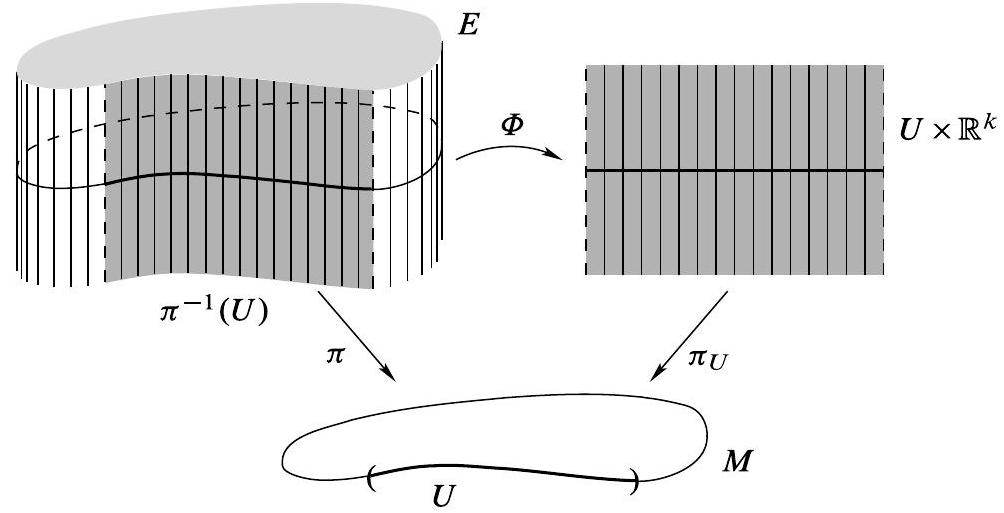
\includegraphics[scale=0.2, center]{2025_06_03_90f64b1a1e243cccc2e0g-268}
Fig. 10.1 A local trivialization of a vector bundle\\



A rank-1 vector bundle is often called a (real) line bundle. Complex vector bundles are defined similarly, with "real vector space" replaced by "complex vector space" and $\mathbb{R}^{k}$ replaced by $\mathbb{C}^{k}$ in the definition. We have no need to treat complex vector bundles in this book, so all of our vector bundles are understood without further comment to be real.

The space $E$ is called the total space of the bundle, $M$ is called its base, and $\pi$ is its projection. Depending on what we wish to emphasize, we sometimes omit some of the ingredients from the notation, and write " $E$ is a vector bundle over $M$," or " $E \rightarrow M$ is a vector bundle," or " $\pi: E \rightarrow M$ is a vector bundle."

\begin{itemize}
  \item Exercise 10.1. Suppose $E$ is a smooth vector bundle over M. Show that the projection map $\pi: E \rightarrow M$ is a surjective smooth submersion.
\end{itemize}

\begin{DEF}{GA-L13-05-02}{Triviales Vektorbündel}
If there exists a local trivialization of $E$ over all of $M$ (called a global trivialization of $\boldsymbol{E}$ ), then $E$ is said to be a trivial bundle. In this case, $E$ itself is homeomorphic to the product space $M \times \mathbb{R}^{k}$. If $E \rightarrow M$ is a smooth bundle that admits a smooth global trivialization, then we say that $E$ is smoothly trivial. In this case $E$ is diffeomorphic to $M \times \mathbb{R}^{k}$, not just homeomorphic.
\end{DEF}

For brevity, when we say that a smooth bundle is trivial, we always understand this to mean smoothly trivial, not just trivial in the topological sense.



Example 10.2 (Product Bundles). 


\begin{EXA}{GA-L13-05-03}{Produkt Vektorbündel als triviales Bündel}
One particularly simple example of a rank$k$ vector bundle over any space $M$ is the product space $E=M \times \mathbb{R}^k$ with $\pi=\pi_1: M \times \mathbb{R}^k \rightarrow M$ as its projection. Any such bundle, called a product bundle, is trivial (with the identity map as a global trivialization). If $M$ is a smooth manifold with or without boundary, then $M \times \mathbb{R}^k$ is smoothly trivial.
\end{EXA}


Although there are many vector bundles that are not trivial, the only one that is easy to visualize is the following.

Example 10.3 (The Möbius Bundle). 


\begin{EXA}{GA-L13-05-04}{Möbiusvektorbündel}
Define an equivalence relation on $\mathbb{R}^2$ by declaring that $(x, y) \sim\left(x^{\prime}, y^{\prime}\right)$ if and only if $\left(x^{\prime}, y^{\prime}\right)=\left(x+n,(-1)^n y\right)$ for some $n \in \mathbb{Z}$. Let $E=\mathbb{R}^2 / \sim$ denote the quotient space, and let $q: \mathbb{R}^2 \rightarrow E$ be the quotient map.

To visualize $E$, let $S$ denote the strip $[0,1] \times \mathbb{R} \subseteq \mathbb{R}^2$. The restriction of $q$ to $S$ is surjective and closed, so it is a quotient map. The only nontrivial identifications made by $\left.q\right|_S$ are on the two boundary lines, so we can think of $E$ as the space obtained from $S$ by giving the right-hand edge a half-twist to turn it upside-down, and then pasting it to the left-hand edge (Fig. 10.2). For any $r>0$, the image under the quotient map $q$ of the rectangle $[0,1] \times[-r, r]$ is a smooth compact manifold with boundary called a Möbius band; you can make a paper model of this space by pasting the ends of a strip of paper together with a half-twist.

Consider the following commutative diagram:
where $\pi_1$ is the projection onto the first factor and $\varepsilon: \mathbb{R} \rightarrow \mathbb{S}^1$ is the smooth covering map $\varepsilon(x)=e^{2 \pi i x}$. Because $\varepsilon \circ \pi_1$ is constant on each equivalence class, it descends to a continuous map $\pi: E \rightarrow \mathbb{S}^1$. A straightforward (if tedious) verification shows that $E$ has a unique smooth manifold structure such that $q$ is a smooth covering map and $\pi: E \rightarrow \mathbb{S}^1$ is a smooth real line bundle over $\mathbb{S}^1$, called the Möbius bundle. (If $U \subseteq \mathbb{S}^1$ is an open subset that is evenly covered by $\varepsilon$, and $\widetilde{U} \subseteq \mathbb{R}$ is a component of $\varepsilon^{-1}(U)$, then $q$ restricts to a homeomorphism from $\tilde{U} \times \mathbb{R}$ to $\pi^{-1}(U)$. Using this, one can construct a homeomorphism from $\pi^{-1}(U)$ to $U \times \mathbb{R}$, which serves as a local trivialization of $E$. These local trivializations can be interpreted as coordinate charts defining the smooth structure on $E$. Problem 10-1 asks you to work out the details. Problem 21-9 suggests a more powerful approach.)
\end{EXA}



The most important examples of vector bundles are tangent bundles.


Proposition 10.4 (The Tangent Bundle as a Vector Bundle). 


\begin{PROP}{GA-L13-05-05}{Tangentialbündel ist ein Vektorbündel von Rang n}
Let $M$ be a smooth $n$-manifold with or without boundary, and let TM be its tangent bundle. With its standard projection map, its natural vector space structure on each fiber, and the topology and smooth structure constructed in Proposition 3.18, TM is a smooth vector bundle of rank $n$ over M.
\end{PROP}


Proof. 

\begin{PROOF}{GA-L13-05-06}{P: Tangentialbündel ist ein Vektorbündel von Rang n}
Given any smooth chart ( $U, \varphi$ ) for $M$ with coordinate functions ( $x^i$ ), define a map $\Phi: \pi^{-1}(U) \rightarrow U \times \mathbb{R}^n$ by
$$
\Phi\left(\left.v^i \frac{\partial}{\partial x^i}\right|_p\right)=\left(p,\left(v^1, \ldots, v^n\right)\right) .
$$
This is linear on fibers and satisfies $\pi_1 \circ \Phi=\pi$. The composite map
$$
\pi^{-1}(U) \xrightarrow{\Phi} U \times \mathbb{R}^n \xrightarrow{\varphi \times \operatorname{Id}_{\mathbb{R}} n} \varphi(U) \times \mathbb{R}^n
$$
is equal to the coordinate map $\tilde{\varphi}$ constructed in Proposition 3.18. Since both $\tilde{\varphi}$ and $\varphi \times \operatorname{Id}_{\mathbb{R}^n}$ are diffeomorphisms, so is $\Phi$. Thus, $\Phi$ satisfies all the conditions for a smooth local trivialization.
\end{PROOF}



Any bundle that is not trivial, of course, requires more than one local trivialization. The next lemma shows that the composition of two smooth local trivializations has a simple form where they overlap.

Lemma 10.5. 


\begin{LEM}{GA-L13-05-07}{Darstellung von Kompositionen von glatten lokalen Trivialisierungen}
Let $\pi: E \rightarrow M$ be a smooth vector bundle of rank $k$ over M. Suppose $\Phi: \pi^{-1}(U) \rightarrow U \times \mathbb{R}^k$ and $\Psi: \pi^{-1}(V) \rightarrow V \times \mathbb{R}^k$ are two smooth local trivializations of $E$ with $U \cap V \neq \varnothing$. There exists a smooth map $\tau: U \cap V \rightarrow \mathrm{GL}(k, \mathbb{R})$ such that the composition $\Phi \circ \Psi^{-1}:(U \cap V) \times \mathbb{R}^k \rightarrow(U \cap V) \times \mathbb{R}^k$ has the form
$$
\Phi \circ \Psi^{-1}(p, v)=(p, \tau(p) v)
$$
where $\tau(p) v$ denotes the usual action of the $k \times k$ matrix $\tau(p)$ on the vector $v \in \mathbb{R}^k$.
\end{LEM}


Proof

\begin{PROOF}{GA-L13-05-08}{P: Darstellung von Kompositionen von glatten lokalen Trivialisierungen}
The following diagram commutes:
\[
\begin{tikzcd}[row sep=large, column sep=large]
& \pi^{-1}(U \cap V) \arrow[dl, "\Psi"'] \arrow[dr, "\Phi"] \arrow[d, "\pi"] & \\
(U \cap V) \times \mathbb{R}^k \arrow[dr, "\pi_1"'] & U \cap V \arrow[d, equal] & (U \cap V) \times \mathbb{R}^k \arrow[dl, "\pi_1"] \\
& U \cap V &
\end{tikzcd}
\]
where the maps on top are to be interpreted as the restrictions of $\Psi$ and $\Phi$ to $\pi^{-1}(U \cap V)$. It follows that $\pi_1 \circ\left(\Phi \circ \Psi^{-1}\right)=\pi_1$, which means that
$$
\Phi \circ \Psi^{-1}(p, v)=(p, \sigma(p, v))
$$
for some smooth map $\sigma:(U \cap V) \times \mathbb{R}^k \rightarrow \mathbb{R}^k$. Moreover, for each fixed $p \in U \cap V$, the map $v \mapsto \sigma(p, v)$ from $\mathbb{R}^k$ to itself is an invertible linear map, so there is a nonsingular $k \times k$ matrix $\tau(p)$ such that $\sigma(p, v)=\tau(p) v$. It remains only to show that the map $\tau: U \cap V \rightarrow \mathrm{GL}(k, \mathbb{R})$ is smooth. This is left to Problem 10-4.
\end{PROOF}


\begin{CONC}{GA-L13-05-09}{Übergangsfunktion zwischen lokalen Trivialisierungen}
The smooth map $\tau: U \cap V \rightarrow \mathrm{GL}(k, \mathbb{R})$ described in this lemma is called the transition function between the local trivializations $\Phi$ and $\Psi$. (This is one of the few situations in smooth manifold theory in which it is traditional to use the word "function" even though the codomain is not $\mathbb{R}$ or $\mathbb{R}^k$.) For example, if $M$ is a smooth manifold and $\Phi$ and $\Psi$ are the local trivializations of $T M$ associated with two different smooth charts, then (3.12) shows that the transition function between them is the Jacobian matrix of the coordinate transition map.
\end{CONC}



\begin{MOT}{GA-L13-05-10}{Spezifikation von glatten Strukturen und Topologie auf Vektorbündeln}
Like the tangent bundle, vector bundles are often most easily described by giving a collection of vector spaces, one for each point of the base manifold. In order to make such a set into a smooth vector bundle, we would first have to construct a manifold topology and a smooth structure on the disjoint union of all the vector spaces, and then construct the local trivializations and show that they have the requisite properties. The next lemma provides a shortcut, by showing that it is sufficient to construct the local trivializations, as long as they overlap with smooth transition functions. (See also Problem 10-6 for a stronger form of this result.)
\end{MOT}

Lemma 10.6 (Vector Bundle Chart Lemma). 

\begin{LEM}{GA-L13-05-11}{Vektorbündel Karten Lemma}
Let $M$ be a smooth manifold with or without boundary, and suppose that for each $p \in M$ we are given a real vector space $E_p$ of some fixed dimension $k$. Let $E=\bigsqcup_{p \in M} E_p$, and let $\pi: E \rightarrow M$ be the map that takes each element of $E_p$ to the point $p$. Suppose furthermore that we are given the following data:
\begin{itemize}
  \item[(i)] eine offene Überdeckung \( \{ U_\alpha \}_{\alpha \in A} \) von \( M \),
  
  \item[(ii)] für jedes \( \alpha \in A \) eine bijektive Abbildung
  \[
  \Phi_\alpha: \pi^{-1}(U_\alpha) \rightarrow U_\alpha \times \mathbb{R}^k,
  \]
  deren Einschränkung auf jede Faser \( E_p \) ein Vektorraum-Isomorphismus
  \[
  E_p \to \{p\} \times \mathbb{R}^k \cong \mathbb{R}^k
  \]
  ist,
  
  \item[(iii)] für alle \( \alpha, \beta \in A \) mit \( U_\alpha \cap U_\beta \neq \varnothing \) eine glatte Abbildung
  \[
  \tau_{\alpha\beta} : U_\alpha \cap U_\beta \to \mathrm{GL}(k, \mathbb{R}),
  \]
  so dass die Übergangsabbildung
  \[
  \Phi_\alpha \circ \Phi_\beta^{-1} : (U_\alpha \cap U_\beta) \times \mathbb{R}^k \rightarrow (U_\alpha \cap U_\beta) \times \mathbb{R}^k
  \]
  die Form hat
  \[
  \Phi_\alpha \circ \Phi_\beta^{-1}(p, v) = \left(p, \tau_{\alpha\beta}(p) v\right).
  \]
\end{itemize}
Then $E$ has a unique topology and smooth structure making it into a smooth manifold with or without boundary and a smooth rank- $k$ vector bundle over M, with $\pi$ as projection and $\left\{\left(U_\alpha, \Phi_\alpha\right)\right\}$ as smooth local trivializations.
\end{LEM}



Proof. 

\begin{PROOF}{GA-L13-05-12}{P: Vektorbündel Karten Lemma}
For each point $p \in M$, choose some $U_\alpha$ containing $p$; choose a smooth chart ( $V_p, \varphi_p$ ) for $M$ such that $p \in V_p \subseteq U_\alpha$; and let $\widehat{V}_p=\varphi_p\left(V_p\right) \subseteq \mathbb{R}^n$ or $\mathbb{H}^n$ (where $n$ is the dimension of $M$ ). Define a map $\tilde{\varphi}_p: \pi^{-1}\left(V_p\right) \rightarrow \widehat{V}_p \times \mathbb{R}^k$ by $\tilde{\varphi}_p=\left(\varphi_p \times \operatorname{Id}_{\mathbb{R}^k}\right) \circ \Phi_{\alpha}$:
$$
\pi^{-1}\left(V_{p}\right) \xrightarrow{\Phi_{\alpha}} V_{p} \times \mathbb{R}^{k} \xrightarrow{\varphi_{p} \times \mathrm{Id}_{\mathbb{R}^{k}}} \widehat{V}_{p} \times \mathbb{R}^{k}
$$

We will show that the collection of all such charts $\left\{\left(\pi^{-1}\left(V_{p}\right), \widetilde{\varphi}_{p}\right): p \in M\right\}$ satisfies the conditions of the smooth manifold chart lemma (Lemma 1.35) or its counterpart for manifolds with boundary (Exercise 1.43), and therefore gives $E$ the structure of a smooth manifold with or without boundary.

As a composition of bijective maps, $\widetilde{\varphi}_{p}$ is bijective onto an open subset of either $\mathbb{R}^{n} \times \mathbb{R}^{k}=\mathbb{R}^{n+k}$ or $\mathbb{H}^{n} \times \mathbb{R}^{k} \approx \mathbb{H}^{n+k}$. For any $p, q \in M$, it is easy to check that
$$
\widetilde{\varphi}_{p}\left(\pi^{-1}\left(V_{p}\right) \cap \pi^{-1}\left(V_{q}\right)\right)=\varphi_{p}\left(V_{p} \cap V_{q}\right) \times \mathbb{R}^{k}
$$
which is open because $\varphi_{p}$ is a homeomorphism onto an open subset of $\mathbb{R}^{n}$ or $\mathbb{H}^{n}$. Wherever two such charts overlap, we have
$$
\widetilde{\varphi}_{p} \circ \widetilde{\varphi}_{q}^{-1}=\left(\varphi_{p} \times \operatorname{Id}_{\mathbb{R}^{k}}\right) \circ \Phi_{\alpha} \circ \Phi_{\beta}^{-1} \circ\left(\varphi_{q} \times \operatorname{Id}_{\mathbb{R}^{k}}\right)^{-1}
$$
Since $\varphi_{p} \times \operatorname{Id}_{\mathbb{R}^{k}}, \varphi_{q} \times \operatorname{Id}_{\mathbb{R}^{k}}$, and $\Phi_{\alpha} \circ \Phi_{\beta}^{-1}$ are diffeomorphisms, the composition is a diffeomorphism. Thus, conditions (i)-(iii) of Lemma 1.35 are satisfied. Because the open cover $\left\{V_{p}: p \in M\right\}$ has a countable subcover, (iv) is satisfied as well.

To check the Hausdorff condition (v), just note that any two points in the same space $E_{p}$ lie in one of the charts we have constructed; while if $\xi \in E_{p}$ and $\eta \in E_{q}$ with $p \neq q$, we can choose $V_{p}$ and $V_{q}$ to be disjoint neighborhoods of $p$ and $q$, so that the sets $\pi^{-1}\left(V_{p}\right)$ and $\pi^{-1}\left(V_{q}\right)$ are disjoint coordinate neighborhoods containing $\xi$ and $\eta$, respectively. Thus we have given $E$ the structure of a smooth manifold with or without boundary.

With respect to this structure, each of the maps $\Phi_{\alpha}$ is a diffeomorphism, because in terms of the coordinate charts $\left(\pi^{-1}\left(V_{p}\right), \widetilde{\varphi}_{p}\right)$ for $E$ and $\left(V_{p} \times \mathbb{R}^{k}, \varphi_{p} \times \operatorname{Id}_{\mathbb{R}^{k}}\right)$ for $V_{p} \times \mathbb{R}^{k}$, the coordinate representation of $\Phi_{\alpha}$ is the identity map. The coordinate representation of $\pi$, with respect to the same chart for $E$ and the chart $\left(V_{p}, \varphi_{p}\right)$ for $M$, is $\pi(x, v)=x$, so $\pi$ is smooth as well. Because each $\Phi_{\alpha}$ maps $E_{p}$ to $\{p\} \times \mathbb{R}^{k}$, it is immediate that $\pi_{1} \circ \Phi_{\alpha}=\pi$, and $\Phi_{\alpha}$ is linear on fibers by hypothesis. Thus, $\Phi_{\alpha}$ satisfies all the conditions for a smooth local trivialization.

The fact that this is the unique such smooth structure follows easily from the requirement that the maps $\Phi_{\alpha}$ be diffeomorphisms onto their images: any smooth structure satisfying the same conditions must include all of the charts we constructed, so it is equal to this one.
\end{PROOF}



Here are some examples showing how the chart lemma can be used to construct new vector bundles from old ones.


Example 10.7 (Whitney Sums). 


\begin{EXA}{GA-L13-05-13}{Whitney Summe von Vektorbündeln}
Given a smooth manifold $M$ and smooth vector bundles $E^{\prime} \rightarrow M$ and $E^{\prime \prime} \rightarrow M$ of ranks $k^{\prime}$ and $k^{\prime \prime}$, respectively, we will construct a new vector bundle over $M$ called the Whitney sum of $\boldsymbol{E}^{\prime}$ and $\boldsymbol{E}^{\prime \prime}$, whose fiber at each $p \in M$ is the direct sum $E_{p}^{\prime} \oplus E_{p}^{\prime \prime}$. The total space is defined as $E^{\prime} \oplus E^{\prime \prime}=$ $\bigsqcup_{p \in M}\left(E_{p}^{\prime} \oplus E_{p}^{\prime \prime}\right)$, with the obvious projection $\pi: E^{\prime} \oplus E^{\prime \prime} \rightarrow M$. For each $p \in M$, choose a neighborhood $U$ of $p$ small enough that there exist local trivializations $\left(U, \Phi^{\prime}\right)$ of $E^{\prime}$ and $\left(U, \Phi^{\prime \prime}\right)$ of $E^{\prime \prime}$, and define $\Phi: \pi^{-1}(U) \rightarrow U \times \mathbb{R}^{k^{\prime}+k^{\prime \prime}}$ by
$$
\Phi\left(v^{\prime}, v^{\prime \prime}\right)=\left(\pi^{\prime}\left(v^{\prime}\right),\left(\pi_{\mathbb{R}^{k^{\prime}}} \circ \Phi^{\prime}\left(v^{\prime}\right), \pi_{\mathbb{R}^{k^{\prime \prime}}} \circ \Phi^{\prime \prime}\left(v^{\prime \prime}\right)\right)\right)
$$
Suppose we are given another such pair of local trivializations $\left(\tilde{U}, \tilde{\Phi}^{\prime}\right)$ and $\left(\tilde{U}, \widetilde{\Phi}^{\prime \prime}\right)$. Let $\tau^{\prime}:(U \cap \tilde{U}) \rightarrow \mathrm{GL}\left(k^{\prime}, \mathbb{R}\right)$ and $\tau^{\prime \prime}:(U \cap \tilde{U}) \rightarrow \mathrm{GL}\left(k^{\prime \prime}, \mathbb{R}\right)$ be the corresponding transition functions. Then the transition function for $E^{\prime} \oplus E^{\prime \prime}$ has the form
$$
\widetilde{\Phi} \circ \Phi^{-1}\left(p,\left(v^{\prime}, v^{\prime \prime}\right)\right)=\left(p, \tau(p)\left(v^{\prime}, v^{\prime \prime}\right)\right)
$$
where $\tau(p)=\tau^{\prime}(p) \oplus \tau^{\prime \prime}(p) \in \mathrm{GL}\left(k^{\prime}+k^{\prime \prime}, \mathbb{R}\right)$ is the block diagonal matrix
$$
\left(\begin{array}{cc}
\tau^{\prime}(p) & 0 \\
0 & \tau^{\prime \prime}(p)
\end{array}\right)
$$
Because this depends smoothly on $p$, it follows from the chart lemma that $E^{\prime} \oplus E^{\prime \prime}$ is a smooth vector bundle over $M$.
\end{EXA}



Example 10.8 (Restriction of a Vector Bundle). 

\begin{EXA}{GA-L13-05-14}{Einschränkungen von Vekotbündeln und umgebende Vektorbündel}
Suppose $\pi: E \rightarrow M$ is a rank- $k$ vector bundle and $S \subseteq M$ is any subset. We define the restriction of $\boldsymbol{E}$ to $\boldsymbol{S}$ to be the set $\left.E\right|_{S}=\bigcup_{p \in S} E_{p}$, with the projection $\left.E\right|_{S} \rightarrow S$ obtained by restricting $\pi$. If $\Phi: \pi^{-1}(U) \rightarrow U \times \mathbb{R}^{k}$ is a local trivialization of $E$ over $U \subseteq M$, it restricts to a bijective map $\left.\Phi\right|_{U}:\left(\left.\pi\right|_{S}\right)^{-1}(U \cap S) \rightarrow(U \cap S) \times \mathbb{R}^{k}$, and it is easy to check that these form local trivializations for a vector bundle structure on $\left.E\right|_{S}$. If $E$ is a smooth vector bundle and $S \subseteq M$ is an immersed or embedded submanifold, it follows easily from the chart lemma that $\left.E\right|_{S}$ is a smooth vector bundle. In particular, if $S \subseteq M$ is a smooth (embedded or immersed) submanifold, then the restricted bundle $\left.T M\right|_{S}$ is called the ambient tangent bundle over M.
\end{EXA}

\section*{Local and Global Sections of Vector Bundles}


\begin{DEF}{GA-L13-05-15}{Schnitt in Vektorbündeln}
Let $\pi: E \rightarrow M$ be a vector bundle. A section of $\boldsymbol{E}$ (sometimes called a cross section) is a section of the map $\pi$, that is, a continuous map $\sigma: M \rightarrow E$ satisfying $\pi \circ \sigma=\operatorname{Id}_{M}$. This means that $\sigma(p)$ is an element of the fiber $E_{p}$ for each $p \in M$.
\end{DEF}

\begin{DEF}{GA-L13-05-16}{Lokale / Globale Schnitt in Vektorbündeln}
More generally, a local section of $\boldsymbol{E}$ is a continuous map $\sigma: U \rightarrow E$ defined on some open subset $U \subseteq M$ and satisfying $\pi \circ \sigma=\operatorname{Id}_{U}$. To emphasize the distinction, a section defined on all of $M$ is sometimes called a global section. Note that a local section of $E$ over $U \subseteq M$ is the same as a global section of the restricted bundle $\left.E\right|_{U}$.
\end{DEF}

\begin{DEF}{GA-L13-05-17}{Glatte Schnitt in Vektorbündeln über glatte Mfk}
If $M$ is a smooth manifold with or without boundary and $E$ is a smooth vector bundle, a smooth (local or global) section of $\boldsymbol{E}$ is one that is a smooth map from its domain to $E$.
\end{DEF}

\begin{DEF}{GA-L13-05-18}{Grober Schnitt in Vektorbündeln}
Just as with vector fields, for some purposes it is useful also to consider maps that would be sections except that they might not be continuous. Thus, we define a rough (local or global) section of $\boldsymbol{E}$ over a set $U \subseteq M$ to be a map $\sigma: U \rightarrow E$ (not necessarily continuous) such that $\pi \circ \sigma=\mathrm{Id}_{U}$. A "section" without further qualification always means a continuous section.
\end{DEF}


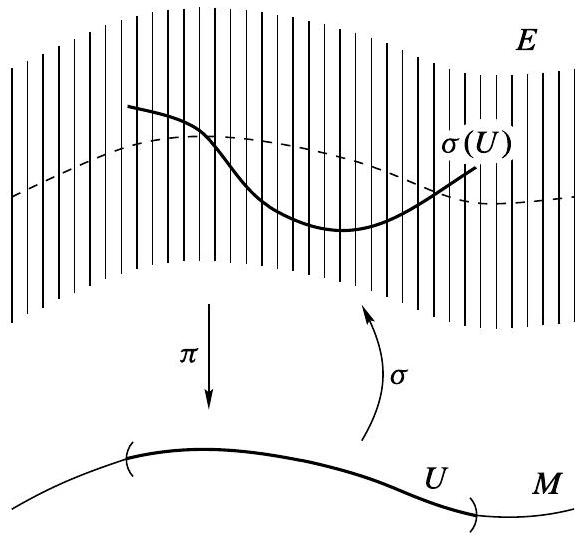
\includegraphics[scale=0.2, center]{2025_06_03_90f64b1a1e243cccc2e0g-274}

Fig. 10.3 A local section of a vector bundle\\


The zero section of $\boldsymbol{E}$ is the global section $\zeta: M \rightarrow E$ defined by

$$
\zeta(p)=0 \in E_{p} \text { for each } p \in M .
$$

As in the case of vector fields, the support of a section $\sigma$ is the closure of the set $\{p \in M: \sigma(p) \neq 0\}$.

Exercise 10.9. Show that the zero section of every vector bundle is continuous, and the zero section of every smooth vector bundle is smooth. [Hint: consider $\Phi \circ \zeta$, where $\Phi$ is a local trivialization.]


Example 10.10 (Sections of Vector Bundles). 

\begin{EXA}{GA-L13-05-19}{Vektorfelder als Schnitte in Tangentialbündel}
Suppose $M$ is a smooth manifold with or without boundary. Sections of $T M$ are vector fields on $M$.
\end{EXA}


\begin{EXA}{GA-L13-05-20}{Vektorfelder entlang von Untermannigfaltigkeiten}
Suppose $M$ is a smooth manifold with or without boundary. Given an immersed submanifold $S \subseteq M$ with or without boundary, a section of the ambient tangent bundle $\left.T M\right|_{S} \rightarrow S$ is called a vector field along $S$. It is a continuous map $X: S \rightarrow T M$ such that $X_{p} \in T_{p} M$ for each $p \in S$. This is different from a vector field on $S$, which satisfies $X_{p} \in T_{p} S$ at each point.
\end{EXA}


\begin{EXA}{GA-L13-05-21}{Schnitte in $E=M \times \mathbb{R}^{k}$}
Suppose $M$ is a smooth manifold with or without boundary. If $E=M \times \mathbb{R}^{k}$ is a product bundle, there is a natural one-to-one correspondence between sections of $E$ and continuous functions from $M$ to $\mathbb{R}^{k}$ : a continuous function $F: M \rightarrow \mathbb{R}^{k}$ determines a section $\widetilde{F}: M \rightarrow M \times \mathbb{R}^{k}$ by $\widetilde{F}(x)=(x, F(x))$, and vice versa. If $M$ is a smooth manifold with or without boundary, then the section $\widetilde{F}$ is smooth if and only if $F$ is.
\end{EXA}


\begin{REM}{GA-L13-05-22}{Natürliche Identifikation von glatten Funktionen und glatten Schnitten im Linienbündel}
Suppose $M$ is a smooth manifold with or without boundary. The correspondence in the preceding paragraph yields a natural identification between the space $C^{\infty}(M)$ and the space of smooth sections of the trivial line bundle $M \times \mathbb{R} \rightarrow M$.
\end{REM}





\begin{PROP}{GA-L13-05-23}{Vektorraum- und Modulstruktur glatter Schnitte}
Sei \( E \rightarrow M \) ein glattes Vektorbündel über einer glatten Mannigfaltigkeit \( M \). Dann ist die Menge \( \Gamma(E) \) der glatten Schnitte von \( E \) ein reeller Vektorraum bezüglich punktweiser Addition und Skalarmultiplikation:
\[
(c_1 \sigma_1 + c_2 \sigma_2)(p) = c_1 \sigma_1(p) + c_2 \sigma_2(p) \quad \text{für alle } p \in M.
\]
Zusätzlich ist \( \Gamma(E) \) ein Modul über dem Ring \( C^\infty(M) \) der glatten, \(\mathbb{R}\)-wertigen Funktionen auf \( M \), wobei die Multiplikation durch \( f \in C^\infty(M) \) gegeben ist durch
\[
(f \cdot \sigma)(p) := f(p) \cdot \sigma(p) \quad \text{für alle } \sigma \in \Gamma(E),\, p \in M.
\]
\end{PROP}




Lemma 10.12 (Extension Lemma for Vector Bundles). 

\begin{LEM}{GA-L13-05-24}{Erweiterungslemma für Vektorbündel}
Let $\pi: E \rightarrow M$ be a smooth vector bundle over a smooth manifold $M$ with or without boundary. Suppose $A$ is a closed subset of $M$, and $\sigma: A \rightarrow E$ is a section of $\left.E\right|_{A}$ that is smooth in the sense that $\sigma$ extends to a smooth local section of $E$ in a neighborhood of each point. For each open subset $U \subseteq M$ containing $A$, there exists a global smooth section $\widetilde{\sigma} \in \Gamma(E)$ such that $\left.\widetilde{\sigma}\right|_{A}=\sigma$ and $\operatorname{supp} \widetilde{\sigma} \subseteq U$.
\begin{itemize}
  \item Exercise 10.13. Prove the preceding lemma.
  \item Exercise 10.14. Let $\pi: E \rightarrow M$ be a smooth vector bundle. Show that each element of $E$ is in the image of a smooth global section.
\end{itemize}
\end{LEM}



\section*{Local and Global Frames}



The concept of local frames that we introduced in Chapter 8 extends readily to vector bundles. 


\begin{DEF}{GA-L13-05-25}{Lokale / Globale Rahmen in Vektorbündeln}
Let $E \rightarrow M$ be a vector bundle. If $U \subseteq M$ is an open subset, a $k$ tuple of local sections $\left(\sigma_{1}, \ldots, \sigma_{k}\right)$ of $E$ over $U$ is said to be linearly independent if their values $\left(\sigma_{1}(p), \ldots, \sigma_{k}(p)\right)$ form a linearly independent $k$-tuple in $E_{p}$ for each $p \in U$. Similarly, they are said to span $\boldsymbol{E}$ if their values span $E_{p}$ for each $p \in U$. A local frame for $\boldsymbol{E}$ over $\boldsymbol{U}$ is an ordered $k$-tuple ( $\sigma_{1}, \ldots, \sigma_{k}$ ) of linearly independent local sections over $U$ that span $E$; thus $\left(\sigma_{1}(p), \ldots, \sigma_{k}(p)\right)$ is a basis for the fiber $E_{p}$ for each $p \in U$. It is called a global frame if $U=M$. If $E \rightarrow M$ is a smooth vector bundle, a local or global frame is a smooth frame if each $\sigma_{i}$ is a smooth section. We often denote a frame ( $\sigma_{1}, \ldots, \sigma_{k}$ ) by ( $\sigma_{i}$ ).
\end{DEF}

The (local or global) frames for $M$ that we defined in Chapter 8 are, in our new terminology, frames for the tangent bundle. We use both terms interchangeably depending on context: "frame for $M$ " and "frame for $T M$ " mean the same thing.

The next proposition is an analogue for vector bundles of Proposition 8.11.

Proposition 10.15 (Completion of Local Frames for Vector Bundles). 

\begin{PROP}{GA-L13-05-26}{Vervollständigung von lokalen Rahmen für Vektorbündel}
Suppose $\pi: E \rightarrow M$ is a smooth vector bundle of rank $k$.\\
\begin{itemize}
  \item[(a)] Ist \( (\sigma_1, \ldots, \sigma_m) \) ein linear unabhängiges \( m \)-Tupel glatter lokaler Schnitte von \( E \) über einer offenen Teilmenge \( U \subseteq M \) mit \( 1 \leq m < k \), so existieren für jeden Punkt \( p \in U \) glatte Schnitte \( \sigma_{m+1}, \ldots, \sigma_k \), definiert auf einer offenen Umgebung \( V \subseteq U \) von \( p \), so dass \( (\sigma_1, \ldots, \sigma_k) \) ein glattes lokales Frame von \( E \) über \( U \cap V \) ist.

  \item[(b)] Ist \( (v_1, \ldots, v_m) \) ein linear unabhängiges \( m \)-Tupel von Vektoren in der Faser \( E_p \) für ein \( p \in M \), mit \( 1 \leq m \leq k \), so existiert ein glattes lokales Frame \( (\sigma_i) \) von \( E \) über einer offenen Umgebung von \( p \), so dass \( \sigma_i(p) = v_i \) für \( i = 1, \ldots, m \).

  \item[(c)] Ist \( A \subseteq M \) eine abgeschlossene Teilmenge und \( (\tau_1, \ldots, \tau_k) \) ein linear unabhängiges \( k \)-Tupel von Schnitten des eingeschränkten Bündels \( E|_A \), die glatt im Sinne von Lemma 10.12 sind, so existiert ein glattes lokales Frame \( (\sigma_1, \ldots, \sigma_k) \) von \( E \) über einer offenen Umgebung von \( A \), so dass \( \sigma_i|_A = \tau_i \) für \( i = 1, \ldots, k \).
\end{itemize}
\end{PROP}


\begin{itemize}
  \item Exercise 10.16. Prove the preceding proposition.
\end{itemize}

Local frames for a vector bundle are intimately connected with local trivializations, as the next two examples show.


Example 10.17 (A Global Frame for a Product Bundle). 


\begin{EXA}{GA-L13-05-27}{Globaler Rahmen für einfache Produktbündel}
If $E=M \times \mathbb{R}^{k} \rightarrow M$ is a product bundle, the standard basis $\left(e_{1}, \ldots, e_{k}\right)$ for $\mathbb{R}^{k}$ yields a global frame $\left(\tilde{e}_{i}\right)$ for $E$, defined by $\tilde{e}_{i}(p)=\left(p, e_{i}\right)$. If $M$ is a smooth manifold with or without boundary, then this global frame is smooth.
\end{EXA}



Example 10.18 (Local Frames Associated with Local Trivializations). 

\begin{EXA}{GA-L13-05-28}{Globaler Rahmen für lokale Trivialisierungen}
Suppose $\pi: E \rightarrow M$ is a smooth vector bundle. If $\Phi: \pi^{-1}(U) \rightarrow U \times \mathbb{R}^{k}$ is a smooth local trivialization of $E$, we can use the same idea as in the preceding example to construct a local frame for $E$ over $U$. Define maps $\sigma_{1}, \ldots, \sigma_{k}: U \rightarrow E$ by $\sigma_{i}(p)=\Phi^{-1}\left(p, e_{i}\right)=\Phi^{-1} \circ \tilde{e}_{i}(p):$
\[
\begin{tikzcd}[row sep=large, column sep=large]
\pi^{-1}(U) \arrow[r, "\Phi"] \arrow[dr, swap, "\pi"] & U \times \mathbb{R}^k \arrow[d, "\pi_1"] \\
& U
\end{tikzcd}
\qquad
\begin{tikzcd}[row sep=large, column sep=huge]
& \pi^{-1}(U) \arrow[dr, "\Phi"] & \\
U \arrow[ur, bend left=20, "\sigma_i"] \arrow[rr, "\widetilde{e}_i", bend left=20] & & U \times \mathbb{R}^k \arrow[ll, "\pi_1"']
\end{tikzcd}
\]
Then $\sigma_{i}$ is smooth because $\Phi$ is a diffeomorphism, and the fact that $\pi_{1} \circ \Phi=\pi$ implies that
$$
\pi \circ \sigma_{i}(p)=\pi \circ \Phi^{-1}\left(p, e_{i}\right)=\pi_{1}\left(p, e_{i}\right)=p,
$$
so $\sigma_{i}$ is a section. 

To see that $\left(\sigma_{i}(p)\right)$ forms a basis for $E_{p}$, just note that $\Phi$ restricts to an isomorphism from $E_{p}$ to $\{p\} \times \mathbb{R}^{k}$, and $\Phi\left(\sigma_{i}(p)\right)=\left(p, e_{i}\right)$, so $\Phi$ takes $\left(\sigma_{i}(p)\right)$ to the standard basis for $\{p\} \times \mathbb{R}^{k} \cong \mathbb{R}^{k}$. We say that this local frame $\left(\sigma_{i}\right)$ is associated with $\boldsymbol{\Phi}$.
\end{EXA}



Proposition 10.19. 

\begin{PROP}{GA-L13-05-29}{Jeder glatter lokaler Rahmen in glatten Vektorbündeln ist mit glatten lokalen Trivialisierungen assoziiert}
Every smooth local frame for a smooth vector bundle is associated with a smooth local trivialization as in Example 10.18.
\end{PROP}


Proof. 

\begin{PROOF}{GA-L13-05-30}{P: Jeder glatter lokaler Rahmen in glatten Vektorbündeln ist mit glatten lokalen Trivialisierungen assoziiert}
Suppose $E \rightarrow M$ is a smooth vector bundle and $\left(\sigma_{i}\right)$ is a smooth local frame for $E$ over an open subset $U \subseteq M$. We define a map $\Psi: U \times \mathbb{R}^{k} \rightarrow \pi^{-1}(U)$ by
$$
\Psi\left(p,\left(v^{1}, \ldots, v^{k}\right)\right)=v^{i} \sigma_{i}(p)
$$
The fact that $\left(\sigma_{i}(p)\right)$ forms a basis for $E_{p}$ at each $p \in U$ implies that $\Psi$ is bijective, and an easy computation shows that $\sigma_{i}=\Psi \circ \tilde{e}_{i}$. Thus, if we can show that $\Psi$ is a diffeomorphism, then $\Psi^{-1}$ will be a smooth local trivialization whose associated local frame is $\left(\sigma_{i}\right)$.

Since $\Psi$ is bijective, to show that it is a diffeomorphism it suffices to show that it is a local diffeomorphism. Given $q \in U$, we can choose a neighborhood $V$ of $q$ in $M$ over which there exists a smooth local trivialization $\Phi: \pi^{-1}(V) \rightarrow V \times \mathbb{R}^{k}$, and by shrinking $V$ if necessary we may assume that $V \subseteq U$. Since $\Phi$ is a diffeomorphism, if we can show that $\left.\Phi \circ \Psi\right|_{V \times \mathbb{R}^{k}}$ is a diffeomorphism from $V \times \mathbb{R}^{k}$ to itself, it follows that $\Psi$ restricts to a diffeomorphism from $V \times \mathbb{R}^{k}$ to $\pi^{-1}(V)$ :
\[
\begin{tikzcd}[column sep=large, row sep=large]
V \times \mathbb{R}^k \arrow[r, "\Psi|_{V \times \mathbb{R}^k}"] \arrow[dr, swap, "\pi_1"] 
  & \pi^{-1}(V) \arrow[r, "\Phi"] \arrow[d, "\pi"] 
  & V \times \mathbb{R}^k \arrow[dl, "\pi_1"] \\
& V
\end{tikzcd}
\]
For each of our smooth sections $\sigma_{i}$, the composite map $\left.\Phi \circ \sigma_{i}\right|_{V}: V \rightarrow V \times \mathbb{R}^{k}$ is smooth, and thus there are smooth functions $\sigma_{i}^{1}, \ldots, \sigma_{i}^{k}: V \rightarrow \mathbb{R}$ such that
$$
\Phi \circ \sigma_{i}(p)=\left(p,\left(\sigma_{i}^{1}(p), \ldots, \sigma_{i}^{k}(p)\right)\right) .
$$
On $V \times \mathbb{R}^{k}$, therefore,
$$
\Phi \circ \Psi\left(p,\left(v^{1}, \ldots, v^{k}\right)\right)=\left(p,\left(v^{i} \sigma_{i}^{1}(p), \ldots, v^{i} \sigma_{i}^{k}(p)\right)\right),
$$
which is clearly smooth.

To show that $(\Phi \circ \Psi)^{-1}$ is smooth, note that the matrix $\left(\sigma_{i}^{j}(p)\right)$ is invertible for each $p$, because $\left(\sigma_{i}(p)\right)$ is a basis for $E_{p}$. Let $\left(\tau_{i}^{j}(p)\right)$ denote the inverse matrix. Because matrix inversion is a smooth map from $\operatorname{GL}(k, \mathbb{R})$ to itself, the functions $\tau_{i}^{j}$ are smooth. It follows from the computations in the preceding paragraph that
$$
(\Phi \circ \Psi)^{-1}\left(p,\left(w^{1}, \ldots, w^{k}\right)\right)=\left(p,\left(w^{i} \tau_{i}^{1}(p), \ldots, w^{i} \tau_{i}^{k}(p)\right)\right),
$$
which is also smooth.
\end{PROOF}




Corollary 10.20. 

\begin{KORO}{GA-L13-05-31}{Glatte Vektorbündel sind glatt trivial gdw wenn glatte globale Schnitte existieren}
A smooth vector bundle is smoothly trivial if and only if it admits a smooth global frame.
\end{KORO}

Proof. 

\begin{PROOF}{GA-L13-05-32}{Glatte Vektorbündel sind glatt trivial gdw wenn glatte globale Schnitte existieren}
Example 10.18 and Proposition 10.19 show that there is a smooth local trivialization over an open subset $U \subseteq M$ if and only if there is a smooth local frame over $U$. The corollary is just the special case of this statement when $U=M$.
\end{PROOF}



\begin{REM}{GA-L13-05-33}{Kriterium für Trivialität von Tangentialbündel}
When applied to the tangent bundle of a smooth manifold $M$, this corollary says that $T M$ is trivial if and only if $M$ is parallelizable. (Recall that in Chapter 8 we defined a parallelizable manifold to be one that admits a smooth global frame for its tangent bundle.)
\end{REM}



Corollary 10.21. 


\begin{KORO}{GA-L13-05-34}{Konstruktion von lokalen Karten von Vektorbündeln aus Karten der Mannigfaltigkeit}
Let $\pi: E \rightarrow M$ be a smooth vector bundle of rank $k$, let ( $V, \varphi$ ) be a smooth chart on $M$ with coordinate functions ( $x^{i}$ ), and suppose there exists a smooth local frame $\left(\sigma_{i}\right)$ for $E$ over $V$. Define $\tilde{\varphi}: \pi^{-1}(V) \rightarrow \varphi(V) \times \mathbb{R}^{k}$ by
$$
\widetilde{\varphi}\left(v^{i} \sigma_{i}(p)\right)=\left(x^{1}(p), \ldots, x^{n}(p), v^{1}, \ldots, v^{k}\right)
$$
Then $\left(\pi^{-1}(V), \widetilde{\varphi}\right)$ is a smooth coordinate chart for $E$.
\end{KORO}


Proof. 


\begin{PROOF}{GA-L13-05-35}{P: Konstruktion von lokalen Karten von Vektorbündeln aus Karten der Mannigfaltigkeit}
Just check that $\widetilde{\varphi}$ is equal to the composition $\left(\varphi \times \operatorname{Id}_{\mathbb{R}^{k}}\right) \circ \Phi$, where $\Phi$ is the local trivialization associated with ( $\sigma_{i}$ ). As a composition of diffeomorphisms, it is a diffeomorphism.
\end{PROOF}

\begin{DEF}{GA-L13-05-36}{Komponentenfunktionen von (groben) Schnitten bzgl lokaler Rahmen}
Just as smoothness of vector fields can be characterized in terms of their component functions in any smooth chart, smoothness of sections of vector bundles can be characterized in terms of local frames. Suppose ( $\sigma_{i}$ ) is a smooth local frame for $E$ over some open subset $U \subseteq M$. If $\tau: M \rightarrow E$ is a rough section, the value of $\tau$ at an arbitrary point $p \in U$ can be written $\tau(p)=\tau^{i}(p) \sigma_{i}(p)$ for some uniquely determined numbers $\left(\tau^{1}(p), \ldots, \tau^{n}(p)\right)$. This defines $k$ functions $\tau^{i}: U \rightarrow \mathbb{R}$, called the component functions of $\tau$ with respect to the given local frame.
\end{DEF}


Proposition 10.22 (Local Frame Criterion for Smoothness). 


\begin{PROP}{GA-L13-05-37}{Lokales Rahmen Kriterium für Glattheit von Schnitten}
Let $\pi: E \rightarrow M$ be a smooth vector bundle, and let $\tau: M \rightarrow E$ be a rough section. If $\left(\sigma_{i}\right)$ is a smooth local frame for $E$ over an open subset $U \subseteq M$, then $\tau$ is smooth on $U$ if and only if its component functions with respect to ( $\sigma_{i}$ ) are smooth.
\end{PROP}



Proof. 


\begin{PROOF}{GA-L13-05-38}{P: Lokales Rahmen Kriterium für Glattheit von Schnitten}
Let $\Phi: \pi^{-1}(U) \rightarrow U \times \mathbb{R}^{k}$ be the local trivialization associated with the local frame ( $\sigma_{i}$ ). Because $\Phi$ is a diffeomorphism, $\tau$ is smooth on $U$ if and only if the composite map $\Phi \circ \tau$ is smooth on $U$. It is straightforward to check that $\Phi \circ \tau(p)=\left(p,\left(\tau^{1}(p), \ldots, \tau^{k}(p)\right)\right)$, where $\left(\tau^{i}\right)$ are the component functions of $\tau$ with respect to $\left(\sigma_{i}\right)$, so $\Phi \circ \tau$ is smooth if and only if the component functions $\tau^{i}$ are smooth.
\begin{itemize}
  \item Exercise 10.23. Let $E \rightarrow M$ be a vector bundle. Show that a rough section of $E$ is continuous if and only if its component functions in each local frame are continuous.
\end{itemize}
\end{PROOF}



Proposition 10.22 applies equally well to local sections, since a local section of $E$ over an open subset $V \subseteq M$ is a global section of the restricted bundle $\left.E\right|_{V}$.



\begin{REM}{GA-L13-05-39}{Zusammenhang zwischen lokalen Rahmen und lokaler Trivialisierung}
The correspondence between local frames and local trivializations leads to the following uniqueness result characterizing the smooth structure on the tangent bundle of a smooth manifold.

Proposition 10.24 (Uniqueness of the Smooth Structure on TM). Let $M$ be a smooth $n$-manifold with or without boundary. The topology and smooth structure on TM constructed in Proposition 3.18 are the unique ones with respect to which $\pi: T M \rightarrow M$ is a smooth vector bundle with the given vector space structure on the fibers, and such that all coordinate vector fields are smooth local sections.
\end{REM}


Proposition 10.24 (Uniqueness of the Smooth Structure on TM). 

\begin{PROP}{GA-L13-05-40}{Eindeutigkeit von glatten Strukturen auf Tangentialbündel}
Let $M$ be a smooth $n$-manifold with or without boundary. The topology and smooth structure on TM constructed in Proposition 3.18 are the unique ones with respect to which $\pi: T M \rightarrow M$ is a smooth vector bundle with the given vector space structure on the fibers, and such that all coordinate vector fields are smooth local sections.
\end{PROP}


Proof. 

\begin{PROOF}{GA-L13-05-41}{Eindeutigkeit von glatten Strukturen auf Tangentialbündel}
Suppose TM is endowed with some topology and smooth structure making it into a smooth vector bundle with the given properties. If $(U, \varphi)$ is any smooth chart for $M$, the corresponding coordinate frame $\left(\partial / \partial x^{i}\right)$ is a smooth local frame over $U$, so by Proposition 10.19 there is a smooth local trivialization $\Phi: \pi^{-1}(U) \rightarrow U \times \mathbb{R}^{n}$ associated with this local frame. Referring back to the construction of Example 10.18, we see that this local trivialization is none other than the map $\Phi$ constructed in Proposition 10.4. It follows from Corollary 10.21 that the natural coordinate chart $\widetilde{\varphi}=\left(\varphi \times \mathrm{Id}_{\mathbb{R}^{n}}\right) \circ \Phi$ belongs to the given smooth structure. Thus, the given smooth structure is equal to the one constructed in Proposition 3.18.
\end{PROOF}



\section*{Bundle Homomorphisms}
If $\pi: E \rightarrow M$ and $\pi^{\prime}: E^{\prime} \rightarrow M^{\prime}$ are vector bundles, a continuous map $F: E \rightarrow E^{\prime}$ is called a bundle homomorphism if there exists a map $f: M \rightarrow M^{\prime}$ satisfying $\pi^{\prime} \circ F=f \circ \pi$,\\
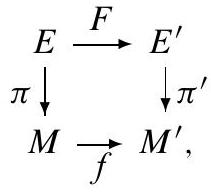
\includegraphics[scale=0.2, center]{2025_06_03_90f64b1a1e243cccc2e0g-279}\\
with the property that for each $p \in M$, the restricted map $\left.F\right|_{E_{p}}: E_{p} \rightarrow E_{f(p)}^{\prime}$ is linear. The relationship between $F$ and $f$ is expressed by saying that $\boldsymbol{F}$ covers $\boldsymbol{f}$.

Proposition 10.25. Suppose $\pi: E \rightarrow M$ and $\pi^{\prime}: E \rightarrow M^{\prime}$ are vector bundles and $F: E \rightarrow E^{\prime}$ is a bundle homomorphism covering $f: M \rightarrow M^{\prime}$. Then $f$ is continuous and is uniquely determined by $F$. If the bundles and $F$ are all smooth, then $f$ is smooth as well.

Proof. All of the conclusions follow from the easily verified fact that $f=\pi^{\prime} \circ F \circ \zeta$, where $\zeta: M \rightarrow E$ is the zero section.

A bijective bundle homomorphism $F: E \rightarrow E^{\prime}$ whose inverse is also a bundle homomorphism is called a bundle isomorphism; if $F$ is also a diffeomorphism, it is called a smooth bundle isomorphism. If there exists a (smooth) bundle isomorphism between $E$ and $E^{\prime}$, the two bundles are said to be (smoothly) isomorphic.

In the special case in which both $E$ and $E^{\prime}$ are vector bundles over the same base space $M$, a slightly more restrictive notion of bundle homomorphism is usually more useful. A bundle homomorphism over $\mathbf{M}$ is a bundle homomorphism covering the identity map of $M$, or in other words, a continuous map $F: E \rightarrow E^{\prime}$ such that $\pi^{\prime} \circ F=\pi$,\\
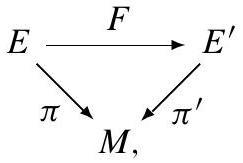
\includegraphics[scale=0.2, center]{2025_06_03_90f64b1a1e243cccc2e0g-279(1)}\\
and whose restriction to each fiber is linear. If there exists a bundle homomorphism $F: E \rightarrow E^{\prime}$ over $M$ that is also a (smooth) bundle isomorphism, then we say that\\
$E$ and $E^{\prime}$ are (smoothly) isomorphic over M. The next proposition shows that it is not necessary to check smoothness of the inverse.

Proposition 10.26. Suppose $E$ and $E^{\prime}$ are smooth vector bundles over a smooth manifold $M$ with or without boundary, and $F: E \rightarrow E^{\prime}$ is a bijective smooth bundle homomorphism over M. Then F is a smooth bundle isomorphism.

Proof. Problem 10-11.\\
Exercise 10.27. Show that a smooth rank- $k$ vector bundle over $M$ is smoothly trivial if and only if it is smoothly isomorphic over $M$ to the product bundle $M \times \mathbb{R}^{k}$.

\section*{Example 10.28 (Bundle Homomorphisms).}
(a) If $F: M \rightarrow N$ is a smooth map, the global differential $d F: T M \rightarrow T N$ is a smooth bundle homomorphism covering $F$.\\
(b) If $E \rightarrow M$ is a smooth vector bundle and $S \subseteq M$ is an immersed submanifold with or without boundary, then the inclusion map $\left.E\right|_{S} \hookrightarrow E$ is a smooth bundle homomorphism covering the inclusion of $S$ into $M$.

Suppose $E \rightarrow M$ and $E^{\prime} \rightarrow M$ are smooth vector bundles over a smooth manifold $M$ with or without boundary, and let $\Gamma(E), \Gamma\left(E^{\prime}\right)$ denote their spaces of smooth global sections. If $F: E \rightarrow E^{\prime}$ is a smooth bundle homomorphism over $M$, then composition with $F$ induces a map $\widetilde{F}: \Gamma(E) \rightarrow \Gamma\left(E^{\prime}\right)$ as follows:

$$
\tilde{F}(\sigma)(p)=(F \circ \sigma)(p)=F(\sigma(p)) .
$$

It is easy to check that $\widetilde{F}(\sigma)$ is a section of $E^{\prime}$, and it is smooth by composition.\\
Because a bundle homomorphism is linear on fibers, the resulting map $\widetilde{F}$ on sections is linear over $\mathbb{R}$. In fact, it satisfies a stronger linearity property. A map $\mathcal{F}: \Gamma(E) \rightarrow \Gamma\left(E^{\prime}\right)$ is said to be linear over $\boldsymbol{C}^{\infty}(\boldsymbol{M})$ if for any smooth functions $u_{1}, u_{2} \in C^{\infty}(M)$ and smooth sections $\sigma_{1}, \sigma_{2} \in \Gamma(E)$,

$$
\mathscr{F}\left(u_{1} \sigma_{1}+u_{2} \sigma_{2}\right)=u_{1} \mathscr{F}\left(\sigma_{1}\right)+u_{2} \mathscr{F}\left(\sigma_{2}\right) .
$$

It follows easily from the definition (10.5) that the map on sections induced by a smooth bundle homomorphism is linear over $C^{\infty}(M)$. The next lemma shows that the converse is true as well.

Lemma 10.29 (Bundle Homomorphism Characterization Lemma). Let $\pi: E \rightarrow$ $M$ and $\pi^{\prime}: E^{\prime} \rightarrow M$ be smooth vector bundles over a smooth manifold $M$ with or without boundary, and let $\Gamma(E), \Gamma\left(E^{\prime}\right)$ denote their spaces of smooth sections. A map $\mathscr{F}: \Gamma(E) \rightarrow \Gamma\left(E^{\prime}\right)$ is linear over $C^{\infty}(M)$ if and only if there is a smooth bundle homomorphism $F: E \rightarrow E^{\prime}$ over $M$ such that $\mathcal{F}(\sigma)=F \circ \sigma$ for all $\sigma \in \Gamma(E)$.

Proof. We noted above that the map on sections induced by a smooth bundle homomorphism is linear over $C^{\infty}(M)$. Conversely, suppose $\mathcal{F}: \Gamma(E) \rightarrow \Gamma\left(E^{\prime}\right)$ is linear over $C^{\infty}(M)$. First, we show that $\mathcal{F}$ acts locally: if $\sigma_{1} \equiv \sigma_{2}$ in some open subset $U \subseteq M$, then $\mathscr{F}\left(\sigma_{1}\right) \equiv \mathscr{F}\left(\sigma_{2}\right)$ in $U$. Write $\tau=\sigma_{1}-\sigma_{2}$; then by linearity of $\mathscr{F}$, it\\
suffices to assume that $\tau$ vanishes in $U$ and show that $\mathscr{F}(\tau)$ does too. Given $p \in U$, let $\psi \in C^{\infty}(M)$ be a smooth bump function supported in $U$ and equal to 1 at $p$. Because $\psi \tau$ is identically zero on $M$, the fact that $\mathscr{F}$ is linear over $C^{\infty}(M)$ implies

$$
0=\mathscr{F}(\psi \tau)=\psi \mathscr{F}(\tau)
$$

Evaluating at $p$ shows that $\mathscr{F}(\tau)(p)=\psi(p) \mathscr{F}(\tau)(p)=0$; since the same is true for every $p \in U$, the claim follows.

Next we show that $\mathcal{F}$ actually acts pointwise: if $\sigma_{1}(p)=\sigma_{2}(p)$, then $\mathcal{F}\left(\sigma_{1}\right)(p)=\mathcal{F}\left(\sigma_{2}\right)(p)$. Once again, it suffices to assume that $\tau(p)=0$ and show that $\mathcal{F}(\tau)(p)=0$. Let $\left(\sigma_{1}, \ldots, \sigma_{k}\right)$ be a smooth local frame for $E$ in some neighborhood $U$ of $p$, and write $\tau$ in terms of this frame as $\tau=u^{i} \sigma_{i}$ for some smooth functions $u^{i}$ defined in $U$. The fact that $\tau(p)=0$ means that $u^{1}(p)=\cdots=u^{k}(p)=0$. By the extension lemmas for vector bundles and for functions, there exist smooth global sections $\tilde{\sigma}_{i} \in \Gamma(E)$ that agree with $\sigma_{i}$ in a neighborhood of $p$, and smooth functions $\tilde{u}^{i} \in C^{\infty}(M)$ that agree with $u^{i}$ in some neighborhood of $p$. Then since $\tau=\tilde{u}^{i} \tilde{\sigma}_{i}$ on a neighborhood of $p$, we have

$$
\mathscr{F}(\tau)(p)=\mathscr{F}\left(\tilde{u}^{i} \tilde{\sigma}_{i}\right)(p)=\tilde{u}^{i}(p) \mathscr{F}\left(\tilde{\sigma}_{i}\right)(p)=0
$$

Define a bundle homomorphism $F: E \rightarrow E^{\prime}$ as follows. For any $p \in M$ and $v \in E_{p}$, let $F(v)=\mathcal{F}(\tilde{v})(p) \in E_{p}^{\prime}$, where $\widetilde{v}$ is any global smooth section of $E$ such that $\tilde{v}(p)=v$. The discussion above shows that the resulting element of $E_{p}^{\prime}$ is independent of the choice of section. This map $F$ clearly satisfies $\pi^{\prime} \circ F=\pi$, and it is linear on each fiber because of the linearity of $\mathcal{F}$. It also satisfies $F \circ \sigma(p)=$ $\mathcal{F}(\sigma)(p)$ for each $\sigma \in \Gamma(E)$ by definition. It remains only to show that $F$ is smooth. It suffices to show that it is smooth in a neighborhood of each point.

Given $p \in M$, let $\left(\sigma_{i}\right)$ be a smooth local frame for $E$ on some neighborhood of $p$. By the extension lemma, there are global sections $\widetilde{\sigma}_{i}$ that agree with $\sigma_{i}$ in a (smaller) neighborhood $U$ of $p$. Shrinking $U$ further if necessary, we may also assume that there exists a smooth local frame $\left(\sigma_{j}^{\prime}\right)$ for $E^{\prime}$ over $U$. Because $\mathcal{F}$ maps smooth global sections of $E$ to smooth global sections of $E^{\prime}$, there are smooth functions $A_{i}^{j} \in C^{\infty}(U)$ such that $\left.\mathscr{F}\left(\widetilde{\sigma}_{i}\right)\right|_{U}=A_{i}^{j} \sigma_{j}^{\prime}$.

For any $q \in U$ and $v \in E_{q}$, we can write $v=v^{i} \sigma_{i}(q)$ for some real numbers $\left(v^{1}, \ldots, v^{k}\right)$, and then

$$
F\left(v^{i} \sigma_{i}(q)\right)=\mathcal{F}\left(v^{i} \widetilde{\sigma}_{i}\right)(q)=v^{i} \mathcal{F}\left(\widetilde{\sigma}_{i}\right)(q)=v^{i} A_{i}^{j}(q) \sigma_{j}^{\prime}(q),
$$

because $v^{i} \widetilde{\sigma}_{i}$ is a global smooth section of $E$ whose value at $q$ is $v$. If $\Phi$ and $\Phi^{\prime}$ denote the local trivializations of $E$ and $E^{\prime}$ associated with the frames $\left(\sigma_{i}\right)$ and $\left(\sigma_{i}^{\prime}\right)$, respectively, it follows that the composite map $\Phi^{\prime} \circ F \circ \Phi^{-1}: U \times \mathbb{R}^{k} \rightarrow U \times \mathbb{R}^{m}$ has the form

$$
\Phi^{\prime} \circ F \circ \Phi^{-1}\left(q,\left(v^{1}, \ldots, v^{k}\right)\right)=\left(q,\left(A_{i}^{1}(q) v^{i}, \ldots, A_{i}^{m}(q) v^{i}\right)\right)
$$

which is smooth. Because $\Phi$ and $\Phi^{\prime}$ are diffeomorphisms, this shows that $F$ is smooth on $\pi^{-1}(U)$.

Later, after we have developed more tools, we will see many examples of smooth bundle homomorphisms. For now, here are some elementary examples.

\section*{Example 10.30 (Bundle Homomorphisms Over Manifolds).}
(a) If $M$ is a smooth manifold and $f \in C^{\infty}(M)$, the map from $\mathfrak{X}(M)$ to itself defined by $X \mapsto f X$ is linear over $C^{\infty}(M)$ because $f\left(u_{1} X_{1}+u_{2} X_{2}\right)=$ $u_{1} f X_{1}+u_{2} f X_{2}$, and thus defines a smooth bundle homomorphism over $M$ from $T M$ to itself.\\
(b) If $Z$ is a smooth vector field on $\mathbb{R}^{3}$, the cross product with $Z$ defines a map from $\mathfrak{X}\left(\mathbb{R}^{3}\right)$ to itself: $X \mapsto X \times Z$. Since it is linear over $C^{\infty}\left(\mathbb{R}^{3}\right)$ in $X$, it determines a smooth bundle homomorphism over $\mathbb{R}^{3}$ from $T \mathbb{R}^{3}$ to $T \mathbb{R}^{3}$.\\
(c) Given $Z \in \mathfrak{X}\left(\mathbb{R}^{n}\right)$, the Euclidean dot product defines a map $X \mapsto X \cdot Z$ from $\mathfrak{X}\left(\mathbb{R}^{n}\right)$ to $C^{\infty}\left(\mathbb{R}^{n}\right)$, which is linear over $C^{\infty}\left(\mathbb{R}^{n}\right)$ and thus determines a smooth bundle homomorphism over $\mathbb{R}^{n}$ from $T \mathbb{R}^{n}$ to the trivial line bundle $\mathbb{R}^{n} \times \mathbb{R}$.\\
//\\
Because of Lemma 10.29, we usually dispense with the notation $\widetilde{F}$ and use the same symbol for both a bundle homomorphism $F: E \rightarrow E^{\prime}$ over $M$ and the linear map $F: \Gamma(E) \rightarrow \Gamma\left(E^{\prime}\right)$ that it induces on sections, and we refer to a map of either of these types as a bundle homomorphism. Because the action on sections is obtained simply by applying the bundle homomorphism pointwise, this should cause no confusion. In fact, we have been doing the same thing all along in certain circumstances. For example, if $a \in \mathbb{R}$, we use the same notation $X \mapsto a X$ to denote both the operation of multiplying vectors in each tangent space $T_{p} M$ by $a$, and the operation of multiplying vector fields by $a$. Because multiplying by $a$ is a bundle homomorphism from $T M$ to itself, there is no ambiguity about what is meant.

It should be noted that most maps that involve differentiation are not bundle homomorphism. For example, if $X$ is a smooth vector field on a smooth manifold $M$, the Lie derivative operator $\mathscr{L}_{X}: \mathfrak{X}(M) \rightarrow \mathfrak{X}(M)$ is not a bundle homomorphism from the tangent bundle to itself, because it is not linear over $C^{\infty}(M)$. As a rule of thumb, a linear map that takes smooth sections of one bundle to smooth sections of another is likely to be a bundle homomorphism if it acts pointwise, but not if it involves differentiation.

\section*{Subbundles}
Given a vector bundle $\pi_{E}: E \rightarrow$ M, a subbundle of $\boldsymbol{E}$ (see Fig. 10.4) is a vector bundle $\pi_{D}: D \rightarrow M$, in which $D$ is a topological subspace of $E$ and $\pi_{D}$ is the restriction of $\pi_{E}$ to $D$, such that for each $p \in M$, the subset $D_{p}=D \cap E_{p}$ is a linear subspace of $E_{p}$, and the vector space structure on $D_{p}$ is the one inherited from $E_{p}$. Note that the condition that $D$ be a vector bundle over $M$ implies that all of the fibers $D_{p}$ must be nonempty and have the same dimension. If $E \rightarrow M$ is a smooth bundle, then a subbundle of $E$ is called a smooth subbundle if it is a smooth vector bundle and an embedded submanifold with or without boundary in $E$.\\
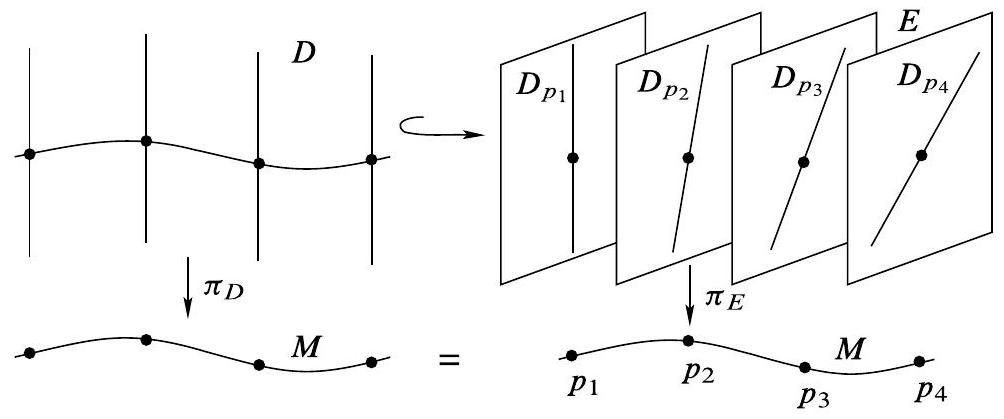
\includegraphics[scale=0.2, center]{2025_06_03_90f64b1a1e243cccc2e0g-283}

Fig. 10.4 A subbundle of a vector bundle

\begin{itemize}
  \item Exercise 10.31. Given a smooth vector bundle $E \rightarrow M$ and a smooth subbundle $D \subseteq E$, show that the inclusion map $\iota: D \hookrightarrow E$ is a smooth bundle homomorphism over $M$.
\end{itemize}

The following lemma gives a convenient condition for checking that a union of subspaces $\left\{D_{p} \subseteq E_{p}: p \in M\right\}$ is a smooth subbundle.

Lemma 10.32 (Local Frame Criterion for Subbundles). Let $\pi: E \rightarrow M$ be a smooth vector bundle, and suppose that for each $p \in M$ we are given an $m$ dimensional linear subspace $D_{p} \subseteq E_{p}$. Then $D=\bigcup_{p \in M} D_{p} \subseteq E$ is a smooth subbundle of $E$ if and only if the following condition is satisfied:

\begin{displayquote}
Each point of $M$ has a neighborhood $U$ on which there exist smooth local sections $\sigma_{1}, \ldots, \sigma_{m}: U \rightarrow E$ with the property that $\sigma_{1}(q), \ldots, \sigma_{m}(q)$ form a basis for $D_{q}$ at each $q \in U$.
\end{displayquote}

Proof. If $D$ is a smooth subbundle, then by definition each $p \in M$ has a neighborhood $U$ over which there exists a smooth local trivialization of $D$, and Example 10.18 shows that there exists a smooth local frame for $D$ over each such set $U$. Such a local frame is by definition a collection of smooth sections $\tau_{1}, \ldots, \tau_{m}: U \rightarrow$ $D$ whose images form a basis for $D_{p}$ at each point $p \in U$. The smooth sections of $E$ that we seek are obtained by composing with the inclusion map $\iota: D \hookrightarrow E$ : $\sigma_{j}=\iota \circ \tau_{j}$.

Conversely, suppose $E \rightarrow M$ is a smooth bundle of rank $k$, and $D \subseteq E$ satisfies (10.6). Each set $D \cap E_{p}$ is a linear subspace of $E_{p}$ by hypothesis, so we need to show that $D$ is an embedded submanifold with or without boundary in $E$ and that the restriction of $\pi$ makes it into a smooth vector bundle over $M$.

To prove that $D$ is an embedded submanifold with or without boundary, it suffices to show that each $p \in M$ has a neighborhood $U$ such that $D \cap \pi^{-1}(U)$ is an embedded submanifold (possibly with boundary) in $\pi^{-1}(U) \subseteq E$. Given $p \in M$, let $\sigma_{1}, \ldots, \sigma_{m}$ be smooth local sections of $E$ satisfying (10.6) on a neighborhood of $p$. By Proposition 10.15, we can complete these to a smooth local frame ( $\sigma_{1}, \ldots, \sigma_{k}$ ) for $E$ over some neighborhood $U$ of $p$. By Proposition 10.19, this local frame is\\
associated with a smooth local trivialization $\Phi: \pi^{-1}(U) \rightarrow U \times \mathbb{R}^{k}$, defined by

$$
\Phi\left(s^{1} \sigma_{1}(q)+\cdots+s^{k} \sigma_{k}(q)\right)=\left(q,\left(s^{1}, \ldots, s^{k}\right)\right) .
$$

This map $\Phi$ takes $D \cap \pi^{-1}(U)$ to the subset $\left\{\left(q,\left(s^{1}, \ldots, s^{m}, 0, \ldots, 0\right)\right)\right\} \subseteq U \times \mathbb{R}^{k}$, which is an embedded submanifold (with boundary if $U$ has a boundary). Moreover, the map $\Psi: D \cap \pi^{-1}(U) \rightarrow U \times \mathbb{R}^{m}$ defined by

$$
\Psi\left(s^{1} \sigma_{1}(q)+\cdots+s^{m} \sigma_{m}(q)\right)=\left(q,\left(s^{1}, \ldots, s^{m}\right)\right)
$$

is a smooth local trivialization of $D$, so $D$ is itself a smooth vector bundle.

\section*{Example 10.33 (Subbundles).}
(a) If $M$ is a smooth manifold and $V$ is a nowhere-vanishing smooth vector field on $M$, then the set $D \subseteq T M$ whose fiber at each $p \in M$ is the linear span of $V_{p}$ is a smooth 1-dimensional subbundle of $T M$.\\
(b) Suppose $E \rightarrow M$ is any trivial bundle, and let ( $E_{1}, \ldots, E_{k}$ ) be a smooth global frame for $E$. If $0 \leq m \leq k$, the subset $D \subseteq E$ defined by $D_{p}=$ span $\left(\left.E_{1}\right|_{p}, \ldots,\left.E_{m}\right|_{p}\right)$ for each $p \in M$ is a smooth subbundle of $E$.\\
(c) Suppose $M$ is a smooth manifold with or without boundary and $S \subseteq M$ is an immersed $k$-submanifold with or without boundary. Problem 10-14 asks you to prove that $T S$ is a smooth rank- $k$ subbundle of the ambient tangent bundle $\left.T M\right|_{S}$.

The next theorem shows how to obtain many more subbundles. Suppose $E \rightarrow M$ and $E^{\prime} \rightarrow M$ are vector bundles and $F: E \rightarrow E^{\prime}$ is a bundle homomorphism over $M$. For each $p \in M$, the rank of the linear map $\left.F\right|_{E_{p}}$ is called the rank of $\boldsymbol{F}$ at $\boldsymbol{p}$. We say that $F$ has constant rank if its rank is the same for all $p \in M$.

Theorem 10.34. Let $E$ and $E^{\prime}$ be smooth vector bundles over a smooth manifold $M$, and let $F: E \rightarrow E^{\prime}$ be a smooth bundle homomorphism over $M$. Define subsets $\operatorname{Ker} F \subseteq E$ and $\operatorname{Im} F \subseteq E^{\prime}$ by

$$
\operatorname{Ker} F=\bigcup_{p \in M} \operatorname{Ker}\left(\left.F\right|_{E_{p}}\right), \quad \operatorname{Im} F=\bigcup_{p \in M} \operatorname{Im}\left(\left.F\right|_{E_{p}}\right)
$$

Then $\operatorname{Ker} F$ and $\operatorname{Im} F$ are smooth subbundles of $E$ and $E^{\prime}$, respectively, if and only if $F$ has constant rank.

Proof. One direction is obvious: since the fibers of a bundle have the same dimension everywhere, the constant-rank condition is certainly necessary for $\operatorname{Ker} F$ and $\operatorname{Im} F$ to be subbundles. To prove sufficiency, suppose $F$ has constant rank $r$, and let $k$ and $k^{\prime}$ be the ranks of the bundles $E$ and $E^{\prime}$, respectively. Let $p \in M$ be arbitrary, and choose a smooth local frame ( $\sigma_{1}, \ldots, \sigma_{k}$ ) for $E$ over a neighborhood $U$ of $p$. For each $i$, the map $F \circ \sigma_{i}: U \rightarrow E^{\prime}$ is a smooth local section of $E^{\prime}$, and these sections span $\left.(\operatorname{Im} F)\right|_{U}$. After rearranging the indices if necessary, we can assume that the elements $\left\{F \circ \sigma_{1}(p), \ldots, F \circ \sigma_{r}(p)\right\}$ form a basis for $\operatorname{Im}\left(\left.F\right|_{E_{p}}\right)$, and by continuity they remain linearly independent in some neighborhood $U_{0}$ of $p$. Since $F$ has\\
constant rank, this means that ( $F \circ \sigma_{1}, \ldots, F \circ \sigma_{r}$ ) forms a smooth local frame for $\operatorname{Im} F$ over $U_{0}$. Since we can do the same in a neighborhood of each point, the local frame criterion shows that $\operatorname{Im} F$ is a smooth subbundle of $E^{\prime}$.

To prove that $\operatorname{Ker} F$ is also a smooth subbundle, let $U_{0}$ and $\left(\sigma_{i}\right)$ be as above, and let $\left.V \subseteq E\right|_{U_{0}}$ be the smooth subbundle spanned by $\sigma_{1}, \ldots, \sigma_{r}$. The smooth bundle homomorphism $\left.F\right|_{V}:\left.V \rightarrow(\operatorname{Im} F)\right|_{U_{0}}$ is bijective, and is thus a smooth bundle isomorphism by Proposition 10.26. Define a smooth bundle homomorphism $\Psi:\left.\left.E\right|_{U_{0}} \rightarrow E\right|_{U_{0}}$ by $\Psi(v)=v-\left(\left.F\right|_{V}\right)^{-1} \circ F(v)$. If $v \in V$, then $F(v)=\left(\left.F\right|_{V}\right)(v)$, so $F(\Psi(v))=F(v)-F \circ\left(\left.F\right|_{V}\right)^{-1} \circ\left(\left.F\right|_{V}\right)(v)=0$. On the other hand, if $v \in$ $\operatorname{Ker} F$, then $\Psi(v)=v$, so again $F(\Psi(v))=F(v)=0$. Since $V$ and $\left.(\operatorname{Ker} F)\right|_{U_{0}}$ together span $\left.E\right|_{U_{0}}$, it follows that $\Psi$ takes its values in $\left.(\operatorname{Ker} F)\right|_{U_{0}}$, and since it restricts to the identity on $\left.(\operatorname{Ker} F)\right|_{U_{0}}$, its image is exactly $\left.(\operatorname{Ker} F)\right|_{U_{0}}$. Thus $\Psi$ has constant rank, and by the argument in the preceding paragraph, $\left.(\operatorname{Ker} F)\right|_{U_{0}}=\operatorname{Im} \Psi$ is a smooth subbundle of $\left.E\right|_{U_{0}}$. Since we can do the same thing in a neighborhood of each point, $\operatorname{Ker} F$ is a smooth subbundle of $E$.

The next proposition illustrates another method for constructing interesting subbundles of the tangent bundle over submanifolds of $\mathbb{R}^{n}$.

Lemma 10.35 (Orthogonal Complement Bundles). Let $M$ be an immersed submanifold with or without boundary in $\mathbb{R}^{n}$, and $D$ be a smooth rank- $k$ subbundle of $\left.T \mathbb{R}^{n}\right|_{M}$. For each $p \in M$, let $D_{p}^{\perp}$ denote the orthogonal complement of $D_{p}$ in $T_{p} \mathbb{R}^{n}$ with respect to the Euclidean dot product, and let $\left.D^{\perp} \subseteq T \mathbb{R}^{n}\right|_{M}$ be the subset

$$
D^{\perp}=\left\{(p, v) \in T \mathbb{R}^{n}: p \in M, v \in D_{p}^{\perp}\right\} .
$$

Then $D^{\perp}$ is a smooth rank- $(n-k)$ subbundle of $\left.T \mathbb{R}^{n}\right|_{M}$. For each $p \in M$, there is a smooth orthonormal frame for $D^{\perp}$ on a neighborhood of $p$.

Proof. Let $p \in M$ be arbitrary, and let ( $X_{1}, \ldots, X_{k}$ ) be a smooth local frame for $D$ over some neighborhood $V$ of $p$ in $M$. Because immersed submanifolds are locally embedded, by shrinking $V$ if necessary, we may assume that it is a single slice in some coordinate ball or half-ball $U \subseteq \mathbb{R}^{n}$. Since $V$ is closed in $U$, Proposition 8.11(c) shows that we can complete ( $X_{1}, \ldots, X_{k}$ ) to a smooth local frame ( $\widetilde{X}_{1}, \ldots, \widetilde{X}_{n}$ ) for $T \mathbb{R}^{n}$ over $U$, and then Lemma 8.13 yields a smooth orthonormal frame $\left(E_{j}\right)$ over $U$ such that $\operatorname{span}\left(\left.E_{1}\right|_{p}, \ldots,\left.E_{k}\right|_{p}\right)=\operatorname{span}\left(\left.X_{1}\right|_{p}, \ldots,\left.X_{k}\right|_{p}\right)=D_{p}$ for each $p \in U$. It follows that ( $E_{k+1}, \ldots, E_{n}$ ) restricts to a smooth orthonormal frame for $D^{\perp}$ over $V$. Thus $D^{\perp}$ satisfies the local frame criterion, and is therefore a smooth subbundle of $\left.T \mathbb{R}^{n}\right|_{M}$.

Corollary 10.36 (The Normal Bundle to a Submanifold of $\mathbb{R}^{\boldsymbol{n}}$ ). If $M \subseteq \mathbb{R}^{\boldsymbol{n}}$ is an immersed m-dimensional submanifold with or without boundary, its normal bundle $N M$ is a smooth rank- $(n-m)$ subbundle of $\left.T \mathbb{R}^{n}\right|_{M}$. For each $p \in M$, there exists a smooth orthonormal frame for NM on a neighborhood of $p$.

Proof. Apply Lemma 10.35 to the smooth subbundle $\left.T M \subseteq T \mathbb{R}^{n}\right|_{M}$.

\section*{Fiber Bundles}
We conclude this chapter by giving a brief introduction to an important generalization of vector bundles, in which the fibers are allowed to be arbitrary topological spaces instead of vector spaces. We can only touch on the subject here; but fiber bundles appear in many applications of manifold theory, so it is important to be at least familiar with the definitions.

Let $M$ and $F$ be topological spaces. A fiber bundle over $M$ with model fiber $\boldsymbol{F}$ is a topological space $E$ together with a surjective continuous map $\pi: E \rightarrow M$ with the property that for each $x \in M$, there exist a neighborhood $U$ of $x$ in $M$ and a homeomorphism $\Phi: \pi^{-1}(U) \rightarrow U \times F$, called a local trivialization of $\boldsymbol{E}$ over $\boldsymbol{U}$, such that the following diagram commutes:\\
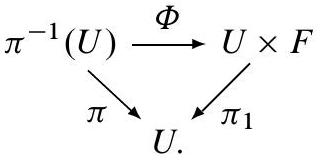
\includegraphics[scale=0.2, center]{2025_06_03_90f64b1a1e243cccc2e0g-286}

The space $E$ is called the total space of the bundle, $M$ is its base, and $\pi$ is its projection. If $E, M$, and $F$ are smooth manifolds with or without boundary, $\pi$ is a smooth map, and the local trivializations can be chosen to be diffeomorphisms, then it is called a smooth fiber bundle.

A trivial fiber bundle is one that admits a local trivialization over the entire base space (a global trivialization). It is said to be smoothly trivial if it is a smooth bundle and the global trivialization is a diffeomorphism.

\section*{Example 10.37 (Fiber Bundles).}
(a) Every product space $M \times F$ is a fiber bundle with projection $\pi_{1}: M \times F \rightarrow M$, called a product fiber bundle. It has a global trivialization given by the identity map $M \times F \rightarrow M \times F$, so every product bundle is trivial.\\
(b) Every rank- $k$ vector bundle is a fiber bundle with model fiber $\mathbb{R}^{k}$.\\
(c) If $E \rightarrow \mathbb{S}^{1}$ is the Möbius bundle of Example 10.3, then the image of $\mathbb{R} \times[-1,1]$ under the quotient map $q: \mathbb{R}^{2} \rightarrow E$ is a fiber bundle over $\mathbb{S}^{1}$ with model fiber $[-1,1]$. It is not a trivial bundle. (Can you prove it?)\\
(d) Every covering map $\pi: E \rightarrow M$ is a fiber bundle whose model fiber is discrete. To construct local trivializations, let $S$ be a discrete space with the same cardinality as the fibers of $\pi$. For each evenly covered open subset $U \subseteq M$, define a map $\Phi: \pi^{-1}(U) \rightarrow U \times S$ by choosing a bijection between the set of components of $\pi^{-1}(U)$ and $S$, and letting $\Phi(x)=(\pi(x), c(x))$, where $c(x)$ is the element of $S$ corresponding to the component containing $x$. //

We will see a few more examples of fiber bundles as we go along.






\pagebreak






\section*{Chapter 12 Tensors}

Much of the technology of smooth manifold theory is designed to allow the concepts of linear algebra to be applied to smooth manifolds. Calculus tells us how to approximate smooth objects by linear ones, and the abstract definitions of manifold theory give a way to interpret these linear approximations in a coordinate-independent way.

In this chapter we carry this idea much further, by generalizing from linear maps to multilinear ones-those that take several vectors as input and depend linearly on each one separately. Although linear maps are paramount in differential geometry, there are many situations in which multilinear maps play important geometric roles. We will introduce a unified language for talking about multilinear maps: the language of tensors. This leads to the concepts of tensors and tensor fields on manifolds.

We begin with tensors on a vector space, which are multilinear generalizations of covectors; a covector is the special case of a tensor of rank one. We give two alternative definitions of tensors on a vector space: on the one hand, they are elements of the abstract "tensor product" of the dual vector space with itself; on the other hand, they are real-valued multilinear functions of several vectors. Each definition is useful in certain contexts. We deal primarily with covariant tensors, but we also give a brief introduction to contravariant tensors and tensors of mixed variance.

Next we introduce two special classes of tensors: the symmetric tensors, whose values are unchanged by permutations of their arguments, and the alternating tensors, whose values change sign when two argument are interchanged.

We then move to smooth manifolds, where we define tensor fields and tensor bundles. After describing the coordinate representations of tensor fields, we describe how they can be pulled back by smooth maps. We also show how the Lie derivative operator can be extended to tensors: the Lie derivative of a tensor field with respect to a vector field is a measure of the rate of change of the tensor field along the flow of the vector field.

Tensors will pervade the rest of the book, and we will see significant applications of them when we study Riemannian metrics, differential forms, orientations, integration, de Rham cohomology, foliations, and symplectic structures.

\section*{Multilinear Algebra}
We have seen some of the important roles played in manifold theory by covectors, which are real-valued linear functions on a vector space. In their simplest form, tensors are just real-valued multilinear functions of one or more variables; simple examples include covectors, inner products, and determinants. To set the stage for our study of tensors, in this section we develop some of the basic properties of multilinear functions in a general setting.

\begin{DEF}{GA-L13-02-01}{Multilineare Abbildung}
Suppose $V_{1}, \ldots, V_{k}$, and $W$ are vector spaces. A map $F: V_{1} \times \cdots \times V_{k} \rightarrow W$ is said to be multilinear if it is linear as a function of each variable separately when the others are held fixed: for each $i$,\\
$F\left(v_{1}, \ldots, a v_{i}+a^{\prime} v_{i}^{\prime}, \ldots, v_{k}\right)=a F\left(v_{1}, \ldots, v_{i}, \ldots, v_{k}\right)+a^{\prime} F\left(v_{1}, \ldots, v_{i}^{\prime}, \ldots, v_{k}\right)$.

(A multilinear function of one variable is just a linear function, and a multilinear function of two variables is generally called bilinear.) Let us write $\mathrm{L}\left(V_{1}, \ldots, V_{k} ; W\right)$ for the set of all multilinear maps from $V_{1} \times \cdots \times V_{k}$ to $W$. It is a vector space under the usual operations of pointwise addition and scalar multiplication:
$$
\begin{aligned}
\left(F+F^{\prime}\right)\left(v_{1}, \ldots, v_{k}\right) & =F\left(v_{1}, \ldots, v_{k}\right)+F^{\prime}\left(v_{1}, \ldots, v_{k}\right) \\
(a F)\left(v_{1}, \ldots, v_{k}\right) & =a\left(F\left(v_{1}, \ldots, v_{k}\right)\right)
\end{aligned}
$$
\end{DEF}





Here are a few examples to keep in mind.



\section*{Example 12.1 (Some Familiar Multilinear Functions).}


\begin{EXA}{GA-L13-02-02}{Dot-Produkt}
The dot product in $\mathbb{R}^{n}$ is a scalar-valued bilinear function of two vectors, used to compute lengths of vectors and angles between them.
\end{EXA}




\begin{EXA}{GA-L13-02-03}{Kreuzprodukt}
The cross product in $\mathbb{R}^{3}$ is a vector-valued bilinear function of two vectors, used to compute areas of parallelograms and to find a third vector orthogonal to two given ones.
\end{EXA}




\begin{EXA}{GA-L13-02-04}{Determinante}
The determinant is a real-valued multilinear function of $n$ vectors in $\mathbb{R}^{n}$, used to detect linear independence and to compute the volume of the parallelepiped spanned by the vectors.
\end{EXA}



\begin{EXA}{GA-L13-02-05}{Lie-Klammer}
The bracket in a Lie algebra g is a g -valued bilinear function of two elements of g .
\end{EXA}


The next example is probably not as familiar, but it is extremely important.


Example 12.2 (Tensor Products of Covectors). 

\begin{EXA}{GA-L13-02-06}{Tensor Produkt für Kovektoren}
Suppose $V$ is a vector space, and $\omega, \eta \in V^{*}$. Define a function $\omega \otimes \eta: V \times V \rightarrow \mathbb{R}$ by
$$
\omega \otimes \eta\left(v_{1}, v_{2}\right)=\omega\left(v_{1}\right) \eta\left(v_{2}\right)
$$
where the product on the right is just ordinary multiplication of real numbers. The linearity of $\omega$ and $\eta$ guarantees that $\omega \otimes \eta$ is a bilinear function of $v_{1}$ and $v_{2}$, so it is an element of $\mathrm{L}(V, V ; \mathbb{R})$. For example, if ( $e^{1}, e^{2}$ ) denotes the standard dual basis for $\left(\mathbb{R}^{2}\right)^{*}$, then $e^{1} \otimes e^{2}: \mathbb{R}^{2} \times \mathbb{R}^{2} \rightarrow \mathbb{R}$ is the bilinear function
$$
e^{1} \otimes e^{2}((w, x),(y, z))=w z
$$
\end{EXA}



\begin{EXA}{GA-L13-02-07}{Tensor Produkt für Multilineare Abbildungen}
The last example can be generalized to arbitrary real-valued multilinear functions as follows: let $V_{1}, \ldots, V_{k}, W_{1}, \ldots, W_{l}$ be real vector spaces, and suppose $F \in \mathrm{~L}\left(V_{1}, \ldots, V_{k} ; \mathbb{R}\right)$ and $G \in \mathrm{~L}\left(W_{1}, \ldots, W_{l} ; \mathbb{R}\right)$. Define a function
$$
F \otimes G: V_{1} \times \cdots \times V_{k} \times W_{1} \times \cdots \times W_{l} \rightarrow \mathbb{R}
$$
by
$$
F \otimes G\left(v_{1}, \ldots, v_{k}, w_{1}, \ldots, w_{l}\right)=F\left(v_{1}, \ldots, v_{k}\right) G\left(w_{1}, \ldots, w_{l}\right)
$$
It follows from the multilinearity of $F$ and $G$ that $F \otimes G\left(v_{1}, \ldots, v_{k}, w_{1}, \ldots, w_{l}\right)$ depends linearly on each argument $v_{i}$ or $w_{j}$ separately, so $F \otimes G$ is an element of $\mathrm{L}\left(V_{1}, \ldots, V_{k}, W_{1}, \ldots, W_{l} ; \mathbb{R}\right)$, called the tensor product of $\boldsymbol{F}$ and $\boldsymbol{G}$.
\end{EXA}



\begin{itemize}
  \item Exercise 12.3. Show that the tensor product operation is bilinear and associative:\\
  $F \otimes G$ depends bilinearly on $F$ and $G$, and $(F \otimes G) \otimes H=F \otimes(G \otimes H)$.\\
\end{itemize}


\begin{PROP}{GA-L13-02-08}{Tensor Produkt für Multilineare Abbildungen ist bilinear und assoziativ}
1. Bilinearität: Das Tensorprodukt $F \otimes G$ hängt bilinear von den beiden Faktoren $F$ und $G$ ab. Das heißt, die Abbildung
$$
(F, G) \mapsto F \otimes G
$$
ist linear in jedem der beiden Argumente, wenn das jeweils andere festgehalten wird. Formal bedeutet das:
$$
\begin{aligned}
\left(\lambda_1 F_1+\lambda_2 F_2\right) \otimes G & =\lambda_1\left(F_1 \otimes G\right)+\lambda_2\left(F_2 \otimes G\right), \\
F \otimes\left(\mu_1 G_1+\mu_2 G_2\right) & =\mu_1\left(F \otimes G_1\right)+\mu_2\left(F \otimes G_2\right),
\end{aligned}
$$
für beliebige Skalare $\lambda_1, \lambda_2, \mu_1, \mu_2$ und beliebige Vektoren (bzw. Tensoren) $F_1, F_2, G_1, G_2$.

2. Assoziativität: Das Tensorprodukt ist assoziativ, d. h. für beliebige Tensoren $F, G, H$ gilt:
$$
(F \otimes G) \otimes H=F \otimes(G \otimes H)
$$
wobei beide Seiten kanonisch als Elemente eines dreifachen Tensorprodukts identifiziert werden. Es gibt also einen natürlichen Isomorphismus
$$
(V \otimes W) \otimes U \cong V \otimes(W \otimes U)
$$
für Vektorräume $V, W, U$, und unter dieser Identifikation stimmen die beiden Tensorprodukte überein.
\end{PROP}



\begin{REM}{GA-L13-02-09}{Notation des Tensorprodukts}
Because of the result of the preceding exercise, we can write tensor products of three or more multilinear functions unambiguously without parentheses. If $F_{1}, \ldots, F_{l}$ are multilinear functions depending on $k_{1}, \ldots, k_{l}$ variables, respectively, their tensor product $F_{1} \otimes \cdots \otimes F_{l}$ is a multilinear function of $k=k_{1}+\cdots+k_{l}$ variables, whose action on $k$ vectors is given by inserting the first $k_{1}$ vectors into $F_{1}$, the next $k_{2}$ vectors into $F_{2}$, and so forth, and multiplying the results together. For example, if $F$ and $G$ are multilinear functions of two vectors and $H$ is a multilinear function of three, then
$$
F \otimes G \otimes H\left(v_{1}, \ldots, v_{7}\right)=F\left(v_{1}, v_{2}\right) G\left(v_{3}, v_{4}\right) H\left(v_{5}, v_{6}, v_{7}\right)
$$
If $\omega^{j} \in V_{j}^{*}$ for $j=1, \ldots, k$, then $\omega^{1} \otimes \cdots \otimes \omega^{k} \in \mathrm{~L}\left(V_{1}, \ldots, V_{k} ; \mathbb{R}\right)$ is the multilinear function given by
$$
\omega^{1} \otimes \cdots \otimes \omega^{k}\left(v_{1}, \ldots, v_{k}\right)=\omega^{1}\left(v_{1}\right) \cdots \omega^{k}\left(v_{k}\right)
$$
\end{REM}



The tensor product operation is important in part because of its role in the following proposition. The notation in this proposition is ugly because of the profusion of indices, but the underlying idea is simple: a basis for any space of multilinear functions can be formed by taking all possible tensor products of basis covectors.


Proposition 12.4 (A Basis for the Space of Multilinear Functions). 


\begin{PROP}{GA-L13-02-10}{Basis für den Raum der multilinearen Abbildungen}
Let $V_{1}, \ldots, V_{k}$ be real vector spaces of dimensions $n_{1}, \ldots, n_{k}$, respectively. For each $j \in\{1, \ldots, k\}$, let $\left(E_{1}^{(j)}, \ldots, E_{n_{j}}^{(j)}\right)$ be a basis for $V_{j}$, and let $\left(\varepsilon_{(j)}^{1}, \ldots, \varepsilon_{(j)}^{n_{j}}\right)$ be the corresponding dual basis for $V_{j}^{*}$. Then the set
$$
\mathcal{B}=\left\{\varepsilon_{(1)}^{i_{1}} \otimes \cdots \otimes \varepsilon_{(k)}^{i_{k}}: 1 \leq i_{1} \leq n_{1}, \ldots, 1 \leq i_{k} \leq n_{k}\right\}
$$
is a basis for $\mathrm{L}\left(V_{1}, \ldots, V_{k} ; \mathbb{R}\right)$, which therefore has dimension equal to $n_{1} \cdots n_{k}$.
\end{PROP}


Proof. 



\begin{PROOF}{GA-L13-02-11}{P: Basis für den Raum der multilinearen Abbildungen}
We need to show that $\mathscr{B}$ is linearly independent and spans $\mathrm{L}\left(V_{1}, \ldots, V_{k} ; \mathbb{R}\right)$. Suppose $F \in \mathrm{~L}\left(V_{1}, \ldots, V_{k} ; \mathbb{R}\right)$ is arbitrary. For each ordered $k$-tuple $\left(i_{1}, \ldots, i_{k}\right)$ of\\
integers with $1 \leq i_{j} \leq n_{j}$, define a number $F_{i_{1} \ldots i_{k}}$ by
$
F_{i_{1} \ldots i_{k}}=F\left(E_{i_{1}}^{(1)}, \ldots, E_{i_{k}}^{(k)}\right)
$
We will show that
$
F=F_{i_{1} \ldots i_{k}} \varepsilon_{(1)}^{i_{1}} \otimes \cdots \otimes \varepsilon_{(k)}^{i_{k}}
$
(with the summation convention in effect as usual), from which it follows that $\mathscr{B}$ spans $\mathrm{L}\left(V_{1}, \ldots, V_{k} ; \mathbb{R}\right)$. For any $k$-tuple of vectors $\left(v_{1}, \ldots, v_{k}\right) \in V_{1} \times \cdots \times V_{k}$, write $v_{1}=v_{1}^{i_{1}} E_{i_{1}}^{(1)}, \ldots, v_{k}=v_{k}^{i_{k}} E_{i_{k}}^{(k)}$, and compute
$
\begin{aligned}
F_{i_{1} \ldots i_{k}} \varepsilon_{(1)}^{i_{1}} \otimes \cdots \otimes \varepsilon_{(k)}^{i_{k}}\left(v_{1}, \ldots, v_{k}\right) & =F_{i_{1} \ldots i_{k}} \varepsilon_{(1)}^{i_{1}}\left(v_{1}\right) \cdots \varepsilon_{(k)}^{i_{k}}\left(v_{k}\right) \\
& =F_{i_{1} \ldots i_{k}} v_{1}^{i_{1}} \cdots v_{k}^{i_{k}}
\end{aligned}
$
while $F\left(v_{1}, \ldots, v_{k}\right)$ is equal to the same thing by multilinearity. This proves the claim.

To show that $\mathscr{B}$ is linearly independent, suppose some linear combination equals zero:
$
F_{i_{1} \ldots i_{k}} \varepsilon_{(1)}^{i_{1}} \otimes \cdots \otimes \varepsilon_{(k)}^{i_{k}}=0
$
Apply this to any ordered $k$-tuple of basis vectors, $\left(E_{j_{1}}^{(1)}, \ldots, E_{j_{k}}^{(k)}\right)$. By the same computation as above, this implies that each coefficient $F_{j_{1} \ldots j_{k}}$ is zero. Thus, the only linear combination of elements of $\mathscr{B}$ that sums to zero is the trivial one.
\end{PROOF}




\begin{CONC}{GA-L13-02-12}{Komponenten von multilinearen Abbildungen durch Anwendung auf Basisvektoren}
This proof shows, by the way, that the components $F_{i_{1} \ldots i_{k}}$ of a multilinear function $F$ in terms of the basis elements in $\mathscr{B}$ are given by
$$F_{i_1 \ldots i_k}=F\left(E_{i_1}^{(1)}, \ldots, E_{i_k}^{(k)}\right)$$
Thus, $F$ is completely determined by its action on all possible sequences of basis vectors.
\end{CONC}



\section*{Abstract Tensor Products of Vector Spaces}


\begin{REM}{GA-L13-02-13}{Konkreter und Abstrakter Zugang zu Tensorprodukt}
The results of the previous section showed that the vector space of multilinear functions $\mathrm{L}\left(V_{1}, \ldots, V_{k} ; \mathbb{R}\right)$ can be viewed as the set of all linear combinations of objects of the form $\omega^{1} \otimes \cdots \otimes \omega^{k}$, where $\omega^{1}, \ldots, \omega^{k}$ are covectors. 

In this section, we give a construction that makes sense of such linear combinations of tensor products in a more abstract setting. The construction is a bit involved, but the idea is simple: given finite-dimensional vector spaces $V_{1}, \ldots, V_{k}$, we will construct a new vector space $V_{1} \otimes \cdots \otimes V_{k}$ whose dimension is the product of the dimensions of the $V_{i}$ 's, and which consists of "formal linear combinations" of objects of the form $v_{1} \otimes \cdots \otimes v_{k}$ for $v_{i} \in V_{i}$, defined in such a way that $v_{1} \otimes \cdots \otimes v_{k}$ depends linearly on each $v_{i}$ separately. (Many of the concepts we introduce in this section-at least the parts that do not refer explicitly to finite bases-work equally well in the infinite-dimensional case; but we mostly restrict our attention to the finite-dimensional case in order to keep things simple.)
\end{REM}

\begin{DEF}{GA-L13-02-14}{Formale Linearkombination und freier Vektorraum}
To begin, we need to make sense of "formal linear combinations." Let $S$ be a set. Roughly speaking, a formal linear combination of elements of $S$ is an expression of the form $\sum_{i=1}^{m} a_{i} x_{i}$, where $a_{1}, \ldots, a_{m}$ are real numbers and $x_{1}, \ldots, x_{m}$ are elements of $S$. 
Of course, since we are not assuming that $S$ has any algebraic structure, we cannot literally add elements of $S$ together or multiply them by numbers. But the essential feature of such an expression is that it is completely determined by which elements of $S$ appear in the sum, and what coefficients appear with them. 

Thus, we make the following definition: for any set $S$, a formal linear combination of elements of $\boldsymbol{S}$ is a function $f: S \rightarrow \mathbb{R}$ such that $f(s)=0$ for all but finitely many $s \in S$. The free (real) vector space on $S$, denoted by $\mathcal{F}(S)$, is the set of all formal linear combinations of elements of $S$. Under pointwise addition and scalar multiplication, $\mathcal{F}(S)$ becomes a vector space over $\mathbb{R}$.

For each element $x \in S$, there is a function $\delta_{x} \in \mathscr{F}(S)$ that takes the value 1 on $x$ and zero on all other elements of $S$; typically we identify this function with $x$ itself, and thus think of $S$ as a subset of $\mathscr{F}(S)$. Every element $f \in \mathscr{F}(S)$ can then be written uniquely in the form $f=\sum_{i=1}^{m} a_{i} x_{i}$, where $x_{1}, \ldots, x_{m}$ are the elements of $S$ for which $f\left(x_{i}\right) \neq 0$, and $a_{i}=f\left(x_{i}\right)$. Thus, $S$ is a basis for $\mathscr{F}(S)$, which is therefore finite-dimensional if and only if $S$ is a finite set.
\end{DEF}

Proposition 12.5 (Characteristic Property of the Free Vector Space). 


\begin{PROP}{GA-L13-02-15}{Erweiterung von Abbildung von Basismenge in Vektorraum für freie Vektorräume}
For any set $S$ and any vector space $W$, every map $A: S \rightarrow W$ has a unique extension to a linear map $\bar{A}: \mathcal{F}(S) \rightarrow W$.
\end{PROP}

\begin{itemize}
  \item Exercise 12.6. Prove the preceding proposition.
\end{itemize}


\begin{DEF}{GA-L13-02-16}{Abstrakte Tensorprodukt via freie Vektorräume}
Now let $V_{1}, \ldots, V_{k}$ be real vector spaces. We begin by forming the free vector space $\mathscr{F}\left(V_{1} \times \cdots \times V_{k}\right)$, which is the set of all finite formal linear combinations of $k$-tuples ( $v_{1}, \ldots, v_{k}$ ) with $v_{i} \in V_{i}$ for $i=1, \ldots, k$. Let $\mathcal{R}$ be the subspace of $\mathcal{F}\left(V_{1} \times \cdots \times V_{k}\right)$ spanned by all elements of the following forms:
$$
\begin{gathered}
\left(v_{1}, \ldots, a v_{i}, \ldots, v_{k}\right)-a\left(v_{1}, \ldots, v_{i}, \ldots, v_{k}\right), \\
\left(v_{1}, \ldots, v_{i}+v_{i}^{\prime}, \ldots, v_{k}\right)-\left(v_{1}, \ldots, v_{i}, \ldots, v_{k}\right)-\left(v_{1}, \ldots, v_{i}^{\prime}, \ldots, v_{k}\right),
\end{gathered}
$$
with $v_{j}, v_{j}^{\prime} \in V_{j}, i \in\{1, \ldots, k\}$, and $a \in \mathbb{R}$.\\
Define the tensor product of the spaces $V_{1}, \ldots, V_{k}$, denoted by $V_{1} \otimes \cdots \otimes V_{k}$, to be the following quotient vector space:
$$
V_{1} \otimes \cdots \otimes V_{k}=\mathscr{F}\left(V_{1} \times \cdots \times V_{k}\right) / \mathscr{R},
$$
and let $\Pi: \mathcal{F}\left(V_{1} \times \cdots \times V_{k}\right) \rightarrow V_{1} \otimes \cdots \otimes V_{k}$ be the natural projection. The equivalence class of an element $\left(v_{1}, \ldots, v_{k}\right)$ in $V_{1} \otimes \cdots \otimes V_{k}$ is denoted by
$$
v_{1} \otimes \cdots \otimes v_{k}=\Pi\left(v_{1}, \ldots, v_{k}\right),
$$
and is called the (abstract) tensor product of $\boldsymbol{v}_{\mathbf{1}}, \ldots, \boldsymbol{v}_{\boldsymbol{k}}$.
\end{DEF}


\begin{REM}{GA-L13-02-17}{Eigenschaften des abstrakten Tensorprodukts}
It follows from the definition that abstract tensor products satisfy
$$
\begin{aligned}
v_{1} \otimes \cdots \otimes a v_{i} \otimes \cdots \otimes v_{k}= & a\left(v_{1} \otimes \cdots \otimes v_{i} \otimes \cdots \otimes v_{k}\right), \\
v_{1} \otimes \cdots \otimes\left(v_{i}+v_{i}^{\prime}\right) \otimes \cdots \otimes v_{k}= & \left(v_{1} \otimes \cdots \otimes v_{i} \otimes \cdots \otimes v_{k}\right) \\
& +\left(v_{1} \otimes \cdots \otimes v_{i}^{\prime} \otimes \cdots \otimes v_{k}\right) .
\end{aligned}
$$
\end{REM}


\begin{REM}{GA-L13-02-18}{todo abstrakte tensorprodukt}
Note that the definition implies that every element of $V_{1} \otimes \cdots \otimes V_{k}$ can be expressed as a linear combination of elements of the form $v_{1} \otimes \cdots \otimes v_{k}$ for $v_{i} \in V_{i}$; but it is not true in general that every element of the tensor product space is of the form $v_{1} \otimes \cdots \otimes v_{k}$ (see Problem 12-1).
\end{REM}

Proposition 12.7 (Characteristic Property of the Tensor Product Space). 


\begin{PROP}{GA-L13-02-19}{Charakteristische Eigenschaften des Tensor Produkt Raumes}
Let $V_{1}, \ldots, V_{k}$ be finite-dimensional real vector spaces. If $A: V_{1} \times \cdots \times V_{k} \rightarrow X$ is any multilinear map into a vector space $X$, then there is a unique linear map $\tilde{A}: V_{1} \otimes \cdots \otimes V_{k} \rightarrow X$ such that the following diagram commutes:\\
\[
\begin{tikzcd}[row sep=large, column sep=large]
V_1 \times \cdots \times V_k \arrow[r, "A"] \arrow[d, "\pi"'] & X \\
V_1 \otimes \cdots \otimes V_k \arrow[ru, dashed, "\widetilde{A}"']
\end{tikzcd}
\]
where $\pi$ is the map $\pi\left(v_{1}, \ldots, v_{k}\right)=v_{1} \otimes \cdots \otimes v_{k}$.
\end{PROP}


Proof. 


\begin{PROOF}{GA-L13-02-20}{P: Charakteristische Eigenschaften des Tensor Produkt Raumes}
First note that any map $A: V_{1} \times \cdots \times V_{k} \rightarrow X$ extends uniquely to a linear map $\bar{A}: \mathcal{F}\left(V_{1} \times \cdots \times V_{k}\right) \rightarrow X$ by the characteristic property of the free vector space. This map is characterized by the fact that $\bar{A}\left(v_{1}, \ldots, v_{k}\right)=A\left(v_{1}, \ldots, v_{k}\right)$ whenever $\left(v_{1}, \ldots, v_{k}\right) \in V_{1} \times \cdots \times V_{k} \subseteq \mathscr{F}\left(V_{1} \times \cdots \times V_{k}\right)$. The fact that $A$ is multilinear means precisely that the subspace $\mathcal{R}$ is contained in the kernel of $\bar{A}$, because
$$
\begin{aligned}
\bar{A}\left(v_{1}, \ldots, a v_{i}, \ldots, v_{k}\right) & =A\left(v_{1}, \ldots, a v_{i}, \ldots, v_{k}\right)=a A\left(v_{1}, \ldots, v_{i}, \ldots, v_{k}\right) \\
& =a \bar{A}\left(v_{1}, \ldots, v_{i}, \ldots, v_{k}\right)=\bar{A}\left(a\left(v_{1}, \ldots, v_{i}, \ldots, v_{k}\right)\right)
\end{aligned}
$$
with a similar computation for the other expression in (12.4). Therefore, $\bar{A}$ descends to a linear map $\tilde{A}: V_{1} \otimes \cdots \otimes V_{k}=\mathscr{F}\left(V_{1} \times \cdots \times V_{k}\right) / \mathcal{R} \rightarrow X$ satisfying $\tilde{A} \circ \Pi=\bar{A}$. Since $\pi$ is equal to the inclusion $V_{1} \times \cdots \times V_{k} \hookrightarrow \mathscr{F}\left(V_{1} \times \cdots \times V_{k}\right)$ followed by $\Pi$, this implies $\tilde{A} \circ \pi=A$, which is (12.6). Uniqueness follows from the fact that every element of $V_{1} \otimes \cdots \otimes V_{k}$ can be written as a linear combination of elements of the form $v_{1} \otimes \cdots \otimes v_{k}$, and $\tilde{A}$ is uniquely determined on such elements by
$$
\tilde{A}\left(v_{1} \otimes \cdots \otimes v_{k}\right)=\bar{A}\left(v_{1}, \ldots, v_{k}\right)=A\left(v_{1}, \ldots, v_{k}\right)
$$
\end{PROOF}



The reason this is called the characteristic property is that it uniquely characterizes the tensor product up to isomorphism; see Problem 12-3.



The next result is an analogue of Proposition 12.4 for abstract tensor product spaces.

Proposition 12.8 (A Basis for the Tensor Product Space). 


\begin{PROP}{GA-L13-02-21}{Basis für den Tensor Produkt Raum}
Suppose $V_{1}, \ldots, V_{k}$ are real vector spaces of dimensions $n_{1}, \ldots, n_{k}$, respectively. For each $j=1, \ldots, k$, suppose $\left(E_{1}^{(j)}, \ldots, E_{n_{j}}^{(j)}\right)$ is a basis for $V_{j}$. Then the set
$$
\mathcal{C}=\left\{E_{i_{1}}^{(1)} \otimes \cdots \otimes E_{i_{k}}^{(k)}: 1 \leq i_{1} \leq n_{1}, \ldots, 1 \leq i_{k} \leq n_{k}\right\}
$$
is a basis for $V_{1} \otimes \cdots \otimes V_{k}$, which therefore has dimension equal to $n_{1} \cdots n_{k}$.
\end{PROP}



Proof. 


\begin{PROOF}{GA-L13-02-22}{P: Basis für den Tensor Produkt Raum}
Elements of the form $v_{1} \otimes \cdots \otimes v_{k}$ span the tensor product space by definition; expanding each $v_{i}$ in such an expression in terms of its basis representation shows that $\mathcal{C}$ spans $V_{1} \otimes \cdots \otimes V_{k}$.

To prove that $\mathcal{C}$ is linearly independent, assume that some linear combination of elements of $\mathscr{C}$ is equal to zero:

$$
a^{i_{1} \ldots i_{k}} E_{i_{1}}^{(1)} \otimes \cdots \otimes E_{i_{k}}^{(k)}=0
$$

For each ordered $k$-tuple of indices ( $m_{1}, \ldots, m_{k}$ ), define a multilinear function $\tau^{m_{1} \ldots m_{k}}: V_{1} \times \cdots \times V_{k} \rightarrow \mathbb{R}$ by

$$
\tau^{m_{1} \ldots m_{k}}\left(v_{1}, \ldots, v_{k}\right)=\varepsilon_{(1)}^{m_{1}}\left(v_{1}\right) \cdots \varepsilon_{(k)}^{m_{k}}\left(v_{k}\right)
$$

where $\left(\varepsilon_{(j)}^{i}\right)$ is the basis for $V_{j}^{*}$ dual to $\left(E_{i}^{(j)}\right)$. Because $\tau^{m_{1} \ldots m_{k}}$ is multilinear, it descends to a linear function $\widetilde{\tau}^{m_{1} \ldots m_{k}}: V_{1} \otimes \cdots \otimes V_{k} \rightarrow \mathbb{R}$ by the characteristic property of the tensor product. It follows that

$$
\begin{aligned}
0 & =\tilde{\tau}^{m_{1} \ldots m_{k}}\left(a^{i_{1} \ldots i_{k}} E_{i_{1}}^{(1)} \otimes \cdots \otimes E_{i_{k}}^{(k)}\right) \\
& =a^{i_{1} \ldots i_{k}} \tau^{m_{1} \ldots m_{k}}\left(E_{i_{1}}^{(1)}, \ldots, E_{i_{k}}^{(k)}\right)=a^{m_{1} \ldots m_{k}}
\end{aligned}
$$

which shows that $\mathscr{C}$ is linearly independent.
\end{PROOF}




Proposition 12.9 (Associativity of Tensor Product Spaces). 



\begin{PROP}{GA-L13-02-23}{Assoziativität von Tensor Produkt Raum}
Let $V_{1}, V_{2}, V_{3}$ be finite-dimensional real vector spaces. There are unique isomorphisms
$$
V_{1} \otimes\left(V_{2} \otimes V_{3}\right) \cong V_{1} \otimes V_{2} \otimes V_{3} \cong\left(V_{1} \otimes V_{2}\right) \otimes V_{3}
$$
under which elements of the forms $v_{1} \otimes\left(v_{2} \otimes v_{3}\right), v_{1} \otimes v_{2} \otimes v_{3}$, and $\left(v_{1} \otimes v_{2}\right) \otimes v_{3}$ all correspond.
\end{PROP}



Proof. 

\begin{PROOF}{GA-L13-02-24}{P: Assoziativität von Tensor Produkt Raum}
We construct the isomorphism $V_{1} \otimes V_{2} \otimes V_{3} \cong\left(V_{1} \otimes V_{2}\right) \otimes V_{3}$; the other one is constructed similarly. The map $\alpha: V_{1} \times V_{2} \times V_{3} \rightarrow\left(V_{1} \otimes V_{2}\right) \otimes V_{3}$ defined by
$$
\alpha\left(v_{1}, v_{2}, v_{3}\right)=\left(v_{1} \otimes v_{2}\right) \otimes v_{3}
$$
is obviously multilinear, and thus by the characteristic property of the tensor product it descends uniquely to a linear map $\widetilde{\alpha}: V_{1} \otimes V_{2} \otimes V_{3} \rightarrow\left(V_{1} \otimes V_{2}\right) \otimes V_{3}$ satisfying $\widetilde{\alpha}\left(v_{1} \otimes v_{2} \otimes v_{3}\right)=\left(v_{1} \otimes v_{2}\right) \otimes v_{3}$ for all $v_{1} \in V_{1}, v_{2} \in V_{2}$, and $v_{3} \in V_{3}$. Because $\left(V_{1} \otimes V_{2}\right) \otimes V_{3}$ is spanned by elements of the form $\left(v_{1} \otimes v_{2}\right) \otimes v_{3}, \tilde{\alpha}$ is surjective, and therefore it is an isomorphism for dimensional reasons. It is clearly the unique such isomorphism, because any other would have to agree with $\tilde{\alpha}$ on the set of all elements of the form $v_{1} \otimes v_{2} \otimes v_{3}$, which spans $V_{1} \otimes V_{2} \otimes V_{3}$.
\end{PROOF}


The connection between tensor products in this abstract setting and the more concrete tensor products of multilinear functionals that we defined earlier is based on the following proposition.

Proposition 12.10 (Abstract vs. Concrete Tensor Products). 

\begin{PROP}{GA-L13-02-25}{Beziehung zwischen abstraktem undkKonkretem Tensor Produkt}
If $V_{1}, \ldots, V_{k}$ are finite-dimensional vector spaces, there is a canonical isomorphism
$$
V_{1}^{*} \otimes \cdots \otimes V_{k}^{*} \cong \mathrm{~L}\left(V_{1}, \ldots, V_{k} ; \mathbb{R}\right)
$$
under which the abstract tensor product defined by 
$$v_1 \otimes \cdots \otimes v_k=\Pi\left(v_1, \ldots, v_k\right)$$
corresponds to the tensor product of covectors defined by
$$\omega^1 \otimes \cdots \otimes \omega^k\left(v_1, \ldots, v_k\right)=\omega^1\left(v_1\right) \cdots \omega^k\left(v_k\right)$$
The connection between tensor products in this abstract setting and the more concrete tensor products of multilinear functionals that we defined earlier is based on the following proposition.
\end{PROP}


Proof. 

\begin{PROOF}{GA-L13-02-26}{P: Beziehung zwischen abstraktem undkKonkretem Tensor Produkt}
First, define a map $\Phi: V_{1}^{*} \times \cdots \times V_{k}^{*} \rightarrow \mathrm{~L}\left(V_{1}, \ldots, V_{k} ; \mathbb{R}\right)$ by
$$
\Phi\left(\omega^{1}, \ldots, \omega^{k}\right)\left(v_{1}, \ldots, v_{k}\right)=\omega^{1}\left(v_{1}\right) \cdots \omega^{k}\left(v_{k}\right)
$$
(There is no implied summation in this formula.) The expression on the right depends linearly on each $v_{i}$, so $\Phi\left(\omega^{1}, \ldots, \omega^{k}\right)$ is indeed an element of the space $\mathrm{L}\left(V_{1}, \ldots, V_{k} ; \mathbb{R}\right)$. It is easy to check that $\Phi$ is multilinear as a function of $\omega^{1}, \ldots, \omega^{k}$, so by the characteristic property it descends uniquely to a linear map $\widetilde{\Phi}$ from $V_{1}^{*} \otimes \cdots \otimes V_{k}^{*}$ to $\mathrm{L}\left(V_{1}, \ldots, V_{k} ; \mathbb{R}\right)$, which satisfies
$$
\widetilde{\Phi}\left(\omega^{1} \otimes \cdots \otimes \omega^{k}\right)\left(v_{1}, \ldots, v_{k}\right)=\omega^{1}\left(v_{1}\right) \cdots \omega^{k}\left(v_{k}\right)
$$
It follows immediately from the definition that $\widetilde{\Phi}$ takes abstract tensor products to tensor products of covectors. It also takes the basis of $V_{1}^{*} \otimes \cdots \otimes V_{k}^{*}$ given by Proposition 12.8 to the basis for $\mathrm{L}\left(V_{1}, \ldots, V_{k} ; \mathbb{R}\right)$ of Proposition 12.4, so it is an isomorphism. (Although we used bases to prove that $\widetilde{\Phi}$ is an isomorphism, $\widetilde{\Phi}$ itself is canonically defined without reference to any basis.)
\end{PROOF}


\begin{CONC}{GA-L13-02-27}{Verwendung des Isomorphismus zwischen abstraktem Tensor Produkt Raum und Vektorraum der Multilinearabbildungen}
Using this canonical isomorphism, we henceforth use the notation $V_{1}^{*} \otimes \cdots \otimes V_{k}^{*}$ to denote either the abstract tensor product space or the space $\mathrm{L}\left(V_{1}, \ldots, V_{k} ; \mathbb{R}\right)$, focusing on whichever interpretation is more convenient for the problem at hand.
\end{CONC}


\begin{CONC}{GA-L13-02-28}{Verwendung der Identifikation von Vektorraum mit dem zweiten dualen Vektorraum für end. dim. Vektorräume}
Since we are assuming the vector spaces are all finite-dimensional, we can also identify each $V_{j}$ with its second dual space $V_{j}^{* *}$, and thereby obtain another canonical identification
$$
V_{1} \otimes \cdots \otimes V_{k} \cong \mathrm{~L}\left(V_{1}^{*}, \ldots, V_{k}^{*} ; \mathbb{R}\right)
$$
\end{CONC}



\pagebreak



\section*{Covariant and Contravariant Tensors on a Vector Space}



\begin{DEF}{GA-L13-03-01}{Kovarianter k-Tensor auf Vektorräumen}
Let $V$ be a finite-dimensional real vector space. If $k$ is a positive integer, a covariant $\boldsymbol{k}$-tensor on $\boldsymbol{V}$ is an element of the $k$-fold tensor product $V^{*} \otimes \cdots \otimes V^{*}$, which we typically think of as a real-valued multilinear function of $k$ elements of $V$ :
$$
\alpha: \underbrace{V \times \cdots \times V}_{k \text { copies }} \rightarrow \mathbb{R}
$$
The number $k$ is called the rank of $\boldsymbol{\alpha}$. A 0-tensor is, by convention, just a real number (a real-valued function depending multilinearly on no vectors!). We denote the vector space of all covariant $k$-tensors on $V$ by the shorthand notation
$$
T^{k}\left(V^{*}\right)=\underbrace{V^{*} \otimes \cdots \otimes V^{*}}_{k \text { copies }}
$$
\end{DEF}



Let us look at some examples.


Example 12.11 (Covariant Tensors). 

\begin{EXA}{GA-L13-03-02}{Lineare Funktionale als korvariante 1-Tensoren}
Let $V$ be a finite-dimensional vector space. Every linear functional $\omega: V \rightarrow \mathbb{R}$ is multilinear, so a covariant 1-tensor is just a covector. Thus, $T^{1}\left(V^{*}\right)$ is equal to $V^{*}$.
\end{EXA}


\begin{EXA}{GA-L13-03-03}{Reell-wertige Bilinearabbildung als kovariante 2 Tensoren}
Let $V$ be a finite-dimensional vector space. A covariant 2-tensor on $V$ is a real-valued bilinear function of two vectors, also called a bilinear form. One example is the dot product on $\mathbb{R}^{n}$. More generally, every inner product is a covariant 2-tensor.
\end{EXA}


\begin{EXA}{GA-L13-03-04}{Determinante als kovarianter k-Tensor}
Let $V$ be a finite-dimensional vector space. The determinant, thought of as a function of $n$ vectors, is a covariant $n$-tensor on $\mathbb{R}^{n}$.
\end{EXA}



For some purposes, it is important to generalize the notion of covariant tensors as follows. 


\begin{DEF}{GA-L13-03-05}{Kontravarianter k-Tensor auf Vektorräumen}
For any finite-dimensional real vector space $V$, we define the space of contravariant tensors on $\boldsymbol{V}$ of rank $\boldsymbol{k}$ to be the vector space
$$
T^{k}(V)=\underbrace{V \otimes \cdots \otimes V}_{k \text { copies }}
$$
In particular, $T^{1}(V)=V$, and by convention $T^{0}(V)=\mathbb{R}$. Because we are assuming that $V$ is finite-dimensional, it is possible to identify this space with the set of multilinear functionals of $k$ covectors:
$$
T^{k}(V) \cong\{\text { multilinear functions } \alpha: \underbrace{V^{*} \times \cdots \times V^{*}}_{k \text { copies }} \rightarrow \mathbb{R}\}
$$
But for most purposes, it is easier to think of contravariant tensors simply as elements of the abstract tensor product space.
\end{DEF}


\begin{DEF}{GA-L13-03-06}{k,l-Tensor auf Vektorräumen}
Even more generally, for any nonnegative integers $k, l$, we define the space of mixed tensors on V of type ( $k, l$ ) as
$$
T^{(k, l)}(V)=\underbrace{V \otimes \cdots \otimes V}_{k \text { copies }} \otimes \underbrace{V^{*} \otimes \cdots \otimes V^{*}}_{l \text { copies }}
$$

Some of these spaces are identical:
$$
\begin{aligned}
& T^{(0,0)}(V)=T^{0}\left(V^{*}\right)=T^{0}(V)=\mathbb{R}, \\
& T^{(0,1)}(V)=T^{1}\left(V^{*}\right)=V^{*}, \\
& T^{(1,0)}(V)=T^{1}(V)=V, \\
& T^{(0, k)}(V)=T^{k}\left(V^{*}\right), \\
& T^{(k, 0)}(V)=T^{k}(V) .
\end{aligned}
$$
\end{DEF}

(Be aware that the notation $T^{(k, l)}(V)$ is not universal. Another notation that is in common use for this space is $T_{l}^{k}(V)$. To make matters worse, some books reverse the roles of $k$ and $l$ in either of these notations; for example, the previous edition of this text used the notation $T_{k}^{l}(V)$ for the space we are here denoting by $T^{(k, l)}(V)$.

We have chosen the notation given here because it is common and nearly always means the same thing. The moral, as usual, is that when you read any differential geometry book, you need to make sure you understand the author's notational conventions.)

\begin{REM}{GA-L13-03-07}{Basis für Tensor Räume}
When $V$ is finite-dimensional, any choice of basis for $V$ automatically yields bases for all of the tensor spaces over $V$. The following corollary follows immediately from Proposition 12.8.
\end{REM}


Corollary 12.12. 

\begin{KORO}{GA-L13-03-08}{Basis für Tensor Räume aus (duale) Basis von Vektorraum }
Let $V$ be an $n$-dimensional real vector space. Suppose ( $E_{i}$ ) is any basis for $V$ and $\left(\varepsilon^{j}\right)$ is the dual basis for $V^{*}$. Then the following sets constitute bases for the tensor spaces over $V$ :
$$
\begin{gathered}
\left\{\varepsilon^{i_{1}} \otimes \cdots \otimes \varepsilon^{i_{k}}: 1 \leq i_{1}, \ldots, i_{k} \leq n\right\} \quad \text { for } T^{k}\left(V^{*}\right) ; \\
\left\{E_{i_{1}} \otimes \cdots \otimes E_{i_{k}}: 1 \leq i_{1}, \ldots, i_{k} \leq n\right\} \quad \text { for } T^{k}(V) ; \\
\left\{E_{i_{1}} \otimes \cdots \otimes E_{i_{k}} \otimes \varepsilon^{j_{1}} \otimes \cdots \otimes \varepsilon^{j_{l}}: 1 \leq i_{1}, \ldots, i_{k}, j_{1}, \ldots, j_{l} \leq n\right\} \quad \text { for } T^{(k, l)}(V) .
\end{gathered}
$$
Therefore, $\operatorname{dim} T^{k}\left(V^{*}\right)=\operatorname{dim} T^{k}(V)=n^{k}$ and $\operatorname{dim} T^{(k, l)}(V)=n^{k+l}$.\\
In particular, once a basis is chosen for $V$, every covariant $k$-tensor $\alpha \in T^{k}\left(V^{*}\right)$ can be written uniquely in the form
$$
\alpha=\alpha_{i_{1} \ldots i_{k}} \varepsilon^{i_{1}} \otimes \cdots \otimes \varepsilon^{i_{k}},
$$
where the $n^{k}$ coefficients $\alpha_{i_{1} \ldots i_{k}}$ are determined by
$$
\alpha_{i_{1} \ldots i_{k}}=\alpha\left(E_{i_{1}}, \ldots, E_{i_{k}}\right) .
$$
\end{KORO}


\begin{EXA}{GA-L13-03-09}{Darstellung der Bilinearformen}
For example, $T^{2}\left(V^{*}\right)$ is the space of bilinear forms on $V$, and every bilinear form can be written as $\beta=\beta_{i j} \varepsilon^{i} \otimes \varepsilon^{j}$ for some uniquely determined $n \times n$ matrix ( $\beta_{i j}$ ).
\end{EXA}

In this book we are concerned primarily with covariant tensors. Thus tensors will always be understood to be covariant unless we explicitly specify otherwise. However, it is important to be aware that contravariant and mixed tensors play important roles in more advanced parts of differential geometry, especially Riemannian geometry.


\pagebreak


\section*{Symmetric and Alternating Tensors}
In general, rearranging the arguments of a covariant tensor need not have any predictable effect on its value. However, some special tensors-the dot product, for example-do not change their values when their arguments are rearranged. Others-notably the determinant-change sign whenever two arguments are interchanged. In this section, we describe two classes of tensors that change in a simple way when their arguments are rearranged: the symmetric ones and the alternating ones.

\section*{Symmetric Tensors}
Let $V$ be a finite-dimensional vector space. A covariant $k$-tensor $\alpha$ on $V$ is said to be symmetric if its value is unchanged by interchanging any pair of arguments:

$$
\alpha\left(v_{1}, \ldots, v_{i}, \ldots, v_{j}, \ldots, v_{k}\right)=\alpha\left(v_{1}, \ldots, v_{j}, \ldots, v_{i}, \ldots, v_{k}\right)
$$

whenever $1 \leq i<j \leq k$.

\begin{itemize}
  \item Exercise 12.13. Show that the following are equivalent for a covariant $k$-tensor $\alpha$ :\\
(a) $\alpha$ is symmetric.\\
(b) For any vectors $v_{1}, \ldots, v_{k} \in V$, the value of $\alpha\left(v_{1}, \ldots, v_{k}\right)$ is unchanged when $v_{1}, \ldots, v_{k}$ are rearranged in any order.\\
(c) The components $\alpha_{i_{1} \ldots i_{k}}$ of $\alpha$ with respect to any basis are unchanged by any permutation of the indices.
\end{itemize}

The set of symmetric covariant $k$-tensors is a linear subspace of the space $T^{k}\left(V^{*}\right)$ of all covariant $k$-tensors on $V$; we denote this subspace by $\Sigma^{k}\left(V^{*}\right)$. There is a natural projection from $T^{k}\left(V^{*}\right)$ to $\Sigma^{k}\left(V^{*}\right)$ defined as follows. First, let $S_{k}$ denote the symmetric group on k elements, that is, the group of permutations of the set $\{1, \ldots, k\}$. Given a $k$-tensor $\alpha$ and a permutation $\sigma \in S_{k}$, we define a new $k$-tensor ${ }^{\sigma} \alpha$ by

$$
{ }^{\sigma} \alpha\left(v_{1}, \ldots, v_{k}\right)=\alpha\left(v_{\sigma(1)}, \ldots, v_{\sigma(k)}\right) .
$$

Note that ${ }^{\tau}\left({ }^{\sigma} \alpha\right)={ }^{\tau \sigma} \alpha$, where $\tau \sigma$ represents the composition of $\tau$ and $\sigma$, that is, $\tau \sigma(i)=\tau(\sigma(i))$. (This is the reason for putting $\sigma$ before $\alpha$ in the notation ${ }^{\sigma} \alpha$, instead of after it.) We define a projection Sym: $T^{k}\left(V^{*}\right) \rightarrow \Sigma^{k}\left(V^{*}\right)$ called symmetrization by

$$
\operatorname{Sym} \alpha=\frac{1}{k!} \sum_{\sigma \in S_{k}}{ }^{\sigma} \alpha .
$$

More explicitly, this means that

$$
(\operatorname{Sym} \alpha)\left(v_{1}, \ldots, v_{k}\right)=\frac{1}{k!} \sum_{\sigma \in S_{k}} \alpha\left(v_{\sigma(1)}, \ldots, v_{\sigma(k)}\right) .
$$

Proposition 12.14 (Properties of Symmetrization). Let $\alpha$ be a covariant tensor on a finite-dimensional vector space.\\
(a) Sym $\alpha$ is symmetric.\\
(b) Sym $\alpha=\alpha$ if and only if $\alpha$ is symmetric.

Proof. Suppose $\alpha \in T^{k}\left(V^{*}\right)$. If $\tau \in S_{k}$ is any permutation, then

$$
\begin{aligned}
(\operatorname{Sym} \alpha)\left(v_{\tau(1)}, \ldots, v_{\tau(k)}\right) & =\frac{1}{k!} \sum_{\sigma \in S_{k}}{ }^{\sigma} \alpha\left(v_{\tau(1)}, \ldots, v_{\tau(k)}\right) \\
& =\frac{1}{k!} \sum_{\sigma \in S_{k}}{ }^{\tau \sigma} \alpha\left(v_{1}, \ldots, v_{k}\right)
\end{aligned}
$$

$$
\begin{aligned}
& =\frac{1}{k!} \sum_{\eta \in S_{k}}{ }^{\eta} \alpha\left(v_{1}, \ldots, v_{k}\right) \\
& =(\operatorname{Sym} \alpha)\left(v_{1}, \ldots, v_{k}\right)
\end{aligned}
$$

where we have substituted $\eta=\tau \sigma$ in the second-to-last line and used the fact that $\eta$ runs over all of $S_{k}$ as $\sigma$ does. This shows that Sym $\alpha$ is symmetric.

If $\alpha$ is symmetric, then it follows from Exercise 12.13(b) that ${ }^{\sigma} \alpha=\alpha$ for every $\sigma \in S_{k}$, so it follows immediately that Sym $\alpha=\alpha$. On the other hand, if Sym $\alpha=\alpha$, then $\alpha$ is symmetric because part (a) shows that $\operatorname{Sym} \alpha$ is.

If $\alpha$ and $\beta$ are symmetric tensors on $V$, then $\alpha \otimes \beta$ is not symmetric in general. However, using the symmetrization operator, it is possible to define a new product that takes a pair of symmetric tensors and yields another symmetric tensor. If $\alpha \in$ $\Sigma^{k}\left(V^{*}\right)$ and $\beta \in \Sigma^{l}\left(V^{*}\right)$, we define their symmetric product to be the ( $k+l$ )tensor $\alpha \beta$ (denoted by juxtaposition with no intervening product symbol) given by

$$
\alpha \beta=\operatorname{Sym}(\alpha \otimes \beta) .
$$

More explicitly, the action of $\alpha \beta$ on vectors $v_{1}, \ldots, v_{k+l}$ is given by

$$
\alpha \beta\left(v_{1}, \ldots, v_{k+l}\right)=\frac{1}{(k+l)!} \sum_{\sigma \in S_{k+l}} \alpha\left(v_{\sigma(1)}, \ldots, v_{\sigma(k)}\right) \beta\left(v_{\sigma(k+1)}, \ldots, v_{\sigma(k+l)}\right) .
$$

\section*{Proposition 12.15 (Properties of the Symmetric Product).}
(a) The symmetric product is symmetric and bilinear: for all symmetric tensors $\alpha$, $\beta, \gamma$ and all $a, b \in \mathbb{R}$,

$$
\begin{aligned}
\alpha \beta & =\beta \alpha \\
(a \alpha+b \beta) \gamma & =a \alpha \gamma+b \beta \gamma=\gamma(a \alpha+b \beta)
\end{aligned}
$$

(b) If $\alpha$ and $\beta$ are covectors, then

$$
\alpha \beta=\frac{1}{2}(\alpha \otimes \beta+\beta \otimes \alpha)
$$

\begin{itemize}
  \item Exercise 12.16. Prove Proposition 12.15.
\end{itemize}

\section*{Alternating Tensors}
We continue to assume that $V$ is a finite-dimensional real vector space. A covariant $k$-tensor $\alpha$ on $V$ is said to be alternating (or antisymmetric or skew-symmetric) if it changes sign whenever two of its arguments are interchanged. This means that for all vectors $v_{1}, \ldots, v_{k} \in V$ and every pair of distinct indices $i, j$ it satisfies

$$
\alpha\left(v_{1}, \ldots, v_{i}, \ldots, v_{j}, \ldots, v_{k}\right)=-\alpha\left(v_{1}, \ldots, v_{j}, \ldots, v_{i}, \ldots, v_{k}\right) .
$$

Alternating covariant $k$-tensors are also variously called exterior forms, multicovectors, or $\boldsymbol{k}$-covectors. The subspace of all alternating covariant $k$-tensors on $V$ is denoted by $\Lambda^{k}\left(V^{*}\right) \subseteq T^{k}\left(V^{*}\right)$.

Recall that for any permutation $\sigma \in S_{k}$, the sign of $\sigma$, denoted by sgn $\sigma$, is equal to +1 if $\sigma$ is even (i.e., can be written as a composition of an even number of transpositions), and -1 if $\sigma$ is odd (see Proposition B.26). The following exercise is an analogue of Exercise 12.13.

\begin{itemize}
  \item Exercise 12.17. Show that the following are equivalent for a covariant $k$-tensor $\alpha$ :\\
(a) $\alpha$ is alternating.\\
(b) For any vectors $v_{1}, \ldots, v_{k}$ and any permutation $\sigma \in S_{k}$,
\end{itemize}

$$
\alpha\left(v_{\sigma(1)}, \ldots, v_{\sigma(k)}\right)=(\operatorname{sgn} \sigma) \alpha\left(v_{1}, \ldots, v_{k}\right) .
$$

(c) With respect to any basis, the components $\alpha_{i_{1} \ldots i_{k}}$ of $\alpha$ change sign whenever two indices are interchanged.

Every 0-tensor (which is just a real number) is both symmetric and alternating, because there are no arguments to interchange. Similarly, every 1-tensor is both symmetric and alternating. An alternating 2-tensor on $V$ is a skew-symmetric bilinear form. It is interesting to note that every covariant 2-tensor $\beta$ can be expressed as a sum of an alternating tensor and a symmetric one, because

$$
\begin{aligned}
\beta(v, w) & =\frac{1}{2}(\beta(v, w)-\beta(w, v))+\frac{1}{2}(\beta(v, w)+\beta(w, v)) \\
& =\alpha(v, w)+\sigma(v, w),
\end{aligned}
$$

where $\alpha(v, w)=\frac{1}{2}(\beta(v, w)-\beta(w, v))$ is an alternating tensor, and $\sigma(v, w)=$ $\frac{1}{2}(\beta(v, w)+\beta(w, v))$ is symmetric. This is not true for tensors of higher rank, as Problem 12-7 shows.

There are analogues of symmetrization and symmetric products that apply to alternating tensors, but we will put off introducing them until Chapter 14, where we will study the properties of alternating tensors in much more detail.



\pagebreak


\section*{Tensors and Tensor Fields on Manifolds}


\begin{DEF}{GA-L13-04-01}{k,l-Tensorbündel auf Mannigfaltigkeit}
Let $M$ be a smooth manifold with or without boundary. We define the bundle of covariant $\boldsymbol{k}$-tensors on $\boldsymbol{M}$ by
$$
T^{k} T^{*} M=\coprod_{p \in M} T^{k}\left(T_{p}^{*} M\right)
$$
Analogously, we define the bundle of contravariant $\boldsymbol{k}$-tensors by
$$
T^{k} T M=\coprod_{p \in M} T^{k}\left(T_{p} M\right)
$$
and the bundle of mixed tensors of type ( $\boldsymbol{k}, \boldsymbol{l}$ ) by
$$
T^{(k, l)} T M=\coprod_{p \in M} T^{(k, l)}\left(T_{p} M\right) .
$$

There are natural identifications
$$
\begin{aligned}
& T^{(0,0)} T M=T^{0} T^{*} M=T^{0} T M=M \times \mathbb{R}, \\
& T^{(0,1)} T M=T^{1} T^{*} M=T^{*} M, \\
& T^{(1,0)} T M=T^{1} T M=T M, \\
& T^{(0, k)} T M=T^{k} T^{*} M, \\
& T^{(k, 0)} T M=T^{k} T M .
\end{aligned}
$$
Any one of these bundles is called a tensor bundle over M. (Thus, the tangent and cotangent bundles are special cases of tensor bundles.)
\end{DEF}


\begin{DEF}{GA-L13-04-02}{k,l-Tensorfelder in Tensorbündeln}
A section of a tensor bundle is called a (covariant, contravariant, or mixed) tensor field on M. A smooth tensor field is a section that is smooth in the usual sense of smooth sections of vector bundles. Using the identifications above, we see that contravariant 1-tensor fields are the same as vector fields, and covariant 1 -tensor fields are covector fields. Because a 0-tensor is just a real number, a 0-tensor field is the same as a continuous real-valued function.

The spaces of smooth sections of these tensor bundles, $\Gamma\left(T^{k} T^{*} M\right), \Gamma\left(T^{k} T M\right)$, and $\Gamma\left(T^{(k, l)} T M\right)$, are infinite-dimensional vector spaces over $\mathbb{R}$, and modules over $C^{\infty}(M)$.
\end{DEF}


\begin{DEF}{GA-L13-04-03}{k,l-Tensorfelder in lokalen Koordinaten}
In any smooth local coordinates $\left(x^{i}\right)$, sections of these bundles can be written (using the summation convention) as
$$
A= \begin{cases}A_{i_{1} \ldots i_{k}} d x^{i_{1}} \otimes \cdots \otimes d x^{i_{k}}, & A \in \Gamma\left(T^{k} T^{*} M\right) \\ A^{i_{1} \ldots i_{k}} \frac{\partial}{\partial x^{i_{1}}} \otimes \cdots \otimes \frac{\partial}{\partial x^{i_{k}}}, & A \in \Gamma\left(T^{k} T M\right) \\ A_{j_{1} \ldots l_{l}}^{i_{1} \ldots i_{k}} \frac{\partial}{\partial x^{i_{1}}} \otimes \cdots \otimes \frac{\partial}{\partial x^{i_{k}}} \otimes d x^{j_{1}} \otimes \cdots \otimes d x^{j_{l}}, & A \in \Gamma\left(T^{(k, l)} T M\right)\end{cases}
$$
The functions $A_{i_{1} \ldots i_{k}}, A^{i_{1} \ldots i_{k}}$, or $A_{j_{1} \ldots i_{l}}^{i_{1} \ldots i_{k}}$ are called the component functions of $\boldsymbol{A}$ in the chosen coordinates.
\end{DEF} 

Because smooth covariant tensor fields occupy most of our attention, we adopt the following shorthand notation for the space of all smooth covariant $k$-tensor fields:
$$
\mathcal{T}^{k}(M)=\Gamma\left(T^{k} T^{*} M\right)
$$


Proposition 12.19 (Smoothness Criteria for Tensor Fields). 


\begin{PROP}{GA-L13-04-04}{Glatteis-Kriterium für Tensorfelder}
Let $M$ be a smooth manifold with or without boundary, and let $A: M \rightarrow T^{(0, k)} T M$ be a rough section. The following are equivalent.
\begin{itemize}
  \item[(a)] $A$ is smooth.
  \item[(b)] In every smooth coordinate chart, the component functions of $A$ are smooth.
  \item[(c)] Each point of $M$ is contained in some coordinate chart in which $A$ has smooth component functions.
  \item[(d)] If $X_1, \ldots, X_k \in \mathfrak{X}(M)$, then the function 
  \[
  A(X_1, \ldots, X_k)(p) = A_p(X_1|_p, \ldots, X_k|_p)
  \]
  is smooth on $M$.
  \item[(e)] Whenever $X_1, \ldots, X_k$ are smooth vector fields defined on some open subset $U \subseteq M$, the function $A(X_1, \ldots, X_k)$ is smooth on $U$.
\end{itemize}
\end{PROP}


\begin{itemize}
  \item Exercise 12.20. Prove Proposition 12.19.
  \item Exercise 12.21. Formulate and prove smoothness criteria analogous to those of Proposition 12.19 for contravariant and mixed tensor fields.
\end{itemize}

Proposition 12.22. 

\begin{PROP}{GA-L13-04-05}{Glattheit und Komponentenformeln für $f A$ und $A \otimes B$}
Suppose $M$ is a smooth manifold with or without boundary, $A \in T^{(0, k)} T M, B \in T^{(0, k)} T M$, and $f \in C^{\infty}(M)$. Then $f A$ and $A \otimes B$ are also smooth tensor fields, whose components in any smooth local coordinate chart are
$$
\begin{aligned}
(f A)_{i_{1} \ldots i_{k}} & =f A_{i_{1} \ldots i_{k}} \\
(A \otimes B)_{i_{1} \ldots i_{k+l}} & =A_{i_{1} \ldots i_{k}} B_{i_{k+1} \ldots i_{k+l}}
\end{aligned}
$$
\end{PROP}

Exercise 12.23. Prove Proposition 12.22.\\



\begin{CONC}{GA-L13-04-08}{Kommentar zu Tensor Charakterisierungs Lemma}
Proposition 12.19(d): If $X_1, \ldots, X_k \in \mathfrak{X}(M)$, then the function 
  \[
  A(X_1, \ldots, X_k)(p) = A_p(X_1|_p, \ldots, X_k|_p)
  \]
is smooth on $M$, shows that if $A$ is a smooth covariant $k$-tensor field on $M$ and $X_{1}, \ldots, X_{k}$ are smooth vector fields, then $A\left(X_{1}, \ldots, X_{k}\right)$ is a smooth realvalued function on $M$. Thus $A$ induces a map

$$
\underbrace{\mathfrak{X}(M) \times \cdots \times \mathfrak{X}(M)}_{k \text { copies }} \rightarrow C^{\infty}(M) .
$$

It is easy to see that this map is multilinear over $\mathbb{R}$. In fact, more is true: it is multilinear over $\boldsymbol{C}^{\infty}(\boldsymbol{M})$, which means that for $f, f^{\prime} \in C^{\infty}(M)$ and $X_{i}, X_{i}^{\prime} \in$ $\mathfrak{X}(M)$, we have

$$
\begin{aligned}
& A\left(X_{1}, \ldots, f X_{i}+f^{\prime} X_{i}^{\prime}, \ldots, X_{k}\right) \\
& \quad=f A\left(X_{1}, \ldots, X_{i}, \ldots, X_{k}\right)+f^{\prime} A\left(X_{1}, \ldots, X_{i}^{\prime}, \ldots, X_{k}\right)
\end{aligned}
$$

This property turns out to be characteristic of smooth tensor fields, as the next lemma shows.
\end{CONC}


Lemma 12.24 (Tensor Characterization Lemma). 



\begin{LEM}{GA-L13-04-06}{Tensor Charakterisierungs Lemma}
A map
$$
\mathcal{A}: \underbrace{\mathfrak{X}(M) \times \cdots \times \mathfrak{X}(M)}_{k \text { copies }} \rightarrow C^{\infty}(M)
$$
is induced by a smooth covariant $k$-tensor field as above if and only if it is multilinear over $C^{\infty}(M)$.
\end{LEM}

Proof. 


\begin{PROOF}{GA-L13-04-07}{P: Tensor Charakterisierungs Lemma}
We already noted that if $A$ is a smooth covariant $k$-tensor field, then the map $\left(X_{1}, \ldots, X_{k}\right) \mapsto A\left(X_{1}, \ldots, X_{k}\right)$ is multilinear over $C^{\infty}(M)$. To prove the converse,\\
we proceed as in the proof of the bundle homomorphism characterization lemma (Lemma 10.29).

Suppose, therefore, that $\mathscr{A}$ is a map as in (12.7), and assume that $\mathscr{A}$ is multilinear over $C^{\infty}(M)$. We show first that $\mathscr{A}$ acts locally. If $X_{i}$ is a smooth vector field that vanishes on a neighborhood $U$ of $p$, we can choose a bump function $\psi$ supported in $U$ such that $\psi(p)=1$; then because $\psi X_{i} \equiv 0$ we have
$$
0=\mathscr{A}\left(X_{1}, \ldots, \psi X_{i}, \ldots, X_{k}\right)(p)=\psi(p) \mathscr{A}\left(X_{1}, \ldots, X_{i}, \ldots, X_{k}\right)(p)
$$
It follows as in the proof of Lemma 10.29 that the value of $\mathscr{A}\left(X_{1}, \ldots, X_{k}\right)$ at $p$ depends only on the values of $X_{1}, \ldots, X_{k}$ in a neighborhood of $p$.

Next we show that $\mathscr{A}$ actually acts pointwise. If $\left.X_{i}\right|_{p}=0$, then in any coordinate chart centered at $p$ we can write $X_{i}=X_{i}^{j} \partial / \partial x^{j}$, where the component functions $X_{i}^{j}$ all vanish at $p$. By the extension lemma for vector fields, we can find global smooth vector fields $E_{j}$ on $M$ such that $E_{j}=\partial / \partial x^{j}$ in some neighborhood of $p$; and similarly the locally defined functions $X_{i}^{j}$ can be extended to global smooth functions $f_{i}^{j}$ on $M$ that agree with $X_{i}^{j}$ in a neighborhood of $p$. It follows from the multilinearity of $\mathscr{A}$ over $C^{\infty}(M)$ and the fact that $f_{i}{ }^{j} E_{j}=X_{i}$ in a neighborhood of $p$ that
$$
\begin{aligned}
\mathscr{A}\left(X_{1}, \ldots, X_{i}, \ldots, X_{k}\right)(p) & =\mathscr{A}\left(X_{1}, \ldots, f_{i}^{j} E_{j}, \ldots, X_{k}\right)(p) \\
& =f_{i}^{j}(p) \mathscr{A}\left(X_{1}, \ldots, E_{j}, \ldots, X_{k}\right)(p)=0
\end{aligned}
$$
It follows by linearity that $\mathcal{A}\left(X_{1}, \ldots, X_{k}\right)$ depends only on the value of $X_{i}$ at $p$.\\
Now we define a rough tensor field $A: M \rightarrow T^{k} T^{*} M$ by
$$
A_{p}\left(v_{1}, \ldots, v_{k}\right)=\mathscr{A}\left(V_{1}, \ldots, V_{k}\right)(p)
$$
for $p \in M$ and $v_{1}, \ldots, v_{k} \in T_{p} M$, where $V_{1}, \ldots, V_{k}$ are any extensions of $v_{1}, \ldots, v_{k}$ to smooth global vector fields on $M$. The discussion above shows that this is independent of the choices of extensions, and the resulting tensor field is smooth by Proposition 12.19(d).
\end{PROOF}



A symmetric tensor field on a manifold (with or without boundary) is simply a covariant tensor field whose value at each point is a symmetric tensor. The symmetric product of two or more tensor fields is defined pointwise, just like the tensor product. Thus, for example, if $A$ and $B$ are smooth covector fields, their symmetric product is the smooth 2-tensor field $A B$, which by Proposition 12.15(b) is given by

$$
A B=\frac{1}{2}(A \otimes B+B \otimes A)
$$

Alternating tensor fields are called differential forms; we will study them in depth beginning in Chapter 14.




\pagebreak


\section*{Pullbacks of Tensor Fields}


Just like covector fields, covariant tensor fields can be pulled back by a smooth map to yield tensor fields on the domain. (This construction works only for covariant tensor fields, which is one reason why we focus most of our attention on the covariant case.)

\begin{DEF}{GA-L13-04-10}{Pullback von Tensorfeldern}
Suppose $F: M \rightarrow N$ is a smooth map. For any point $p \in M$ and any $k$-tensor $\alpha \in T^{k}\left(T_{F(p)}^{*} N\right)$, we define a tensor $d F_{p}^{*}(\alpha) \in T^{k}\left(T_{p}^{*} M\right)$, called the pointwise pullback of $\alpha$ by $F$ at $p$, by
$$
d F_{p}^{*}(\alpha)\left(v_{1}, \ldots, v_{k}\right)=\alpha\left(d F_{p}\left(v_{1}\right), \ldots, d F_{p}\left(v_{k}\right)\right)
$$
for any $v_{1}, \ldots, v_{k} \in T_{p} M$. If $A$ is a covariant $k$-tensor field on $N$, we define a rough $k$-tensor field $F^{*} A$ on $M$, called the pullback of $\boldsymbol{A}$ by $\boldsymbol{F}$, by
$$
\left(F^{*} A\right)_{p}=d F_{p}^{*}\left(A_{F(p)}\right)
$$

This tensor field acts on vectors $v_{1}, \ldots, v_{k} \in T_{p} M$ by
$$
\left(F^{*} A\right)_{p}\left(v_{1}, \ldots, v_{k}\right)=A_{F(p)}\left(d F_{p}\left(v_{1}\right), \ldots, d F_{p}\left(v_{k}\right)\right)
$$
\end{DEF}


Proposition 12.25 (Properties of Tensor Pullbacks). 


\begin{PROP}{GA-L13-04-09}{Eigenschaften des Pullbacks von Tensorfeldern }
Suppose $F: M \rightarrow N$ and $G: N \rightarrow P$ are smooth maps, $A$ and $B$ are covariant tensor fields on $N$, and $f$ is a real-valued function on $N$.\\
\begin{itemize}
  \item[(a)] \( F^{*}(f B) = (f \circ F) \, F^{*} B \).
  \item[(b)] \( F^{*}(A \otimes B) = F^{*} A \otimes F^{*} B \).
  \item[(c)] \( F^{*}(A + B) = F^{*} A + F^{*} B \).
  \item[(d)] \( F^{*} B \) ist ein (stetiges) Tensorfeld und glatt, falls \( B \) glatt ist.
  \item[(e)] \( (G \circ F)^{*} B = F^{*}(G^{*} B) \).
  \item[(f)] \( (\mathrm{Id}_{N})^{*} B = B \).
\end{itemize}
\end{PROP}


\begin{itemize}
  \item Exercise 12.26. Prove Proposition 12.25.
\end{itemize}

If $f$ is a continuous real-valued function (i.e., a 0-tensor field) and $B$ is a $k$ tensor field, then it is consistent with our definitions to interpret $f \otimes B$ as $f B$, and $F^{*} f$ as $f \circ F$. With these interpretations, property (a) of the preceding proposition is really just a special case of (b).



\begin{itemize}
  \item Exercise 12.27. Suppose $F: M \rightarrow N$ is a smooth map and $A, B$ are symmetric tensor fields on $N$. Show that $F^{*} A$ and $F^{*} B$ are symmetric, and $F^{*}(A B)=$ $\left(F^{*} A\right)\left(F^{*} B\right)$.
\end{itemize}

The following corollary is an immediate consequence of Proposition 12.25.\\


Corollary 12.28. 

\begin{KORO}{GA-L13-04-11}{Lokale Darstellung des Pullbacks von Tensorfeldern}
Let $F: M \rightarrow N$ be smooth, and let $B$ be a covariant $k$-tensor field on $N$. If $p \in M$ and $\left(y^{i}\right)$ are smooth coordinates for $N$ on a neighborhood of $F(p)$, then $F^{*} B$ has the following expression in a neighborhood of $p$ :
$$
\begin{aligned}
& F^{*}\left(B_{i_{1} \ldots i_{k}} d y^{i_{1}} \otimes \cdots \otimes d y^{i_{k}}\right) \\
& \quad=\left(B_{i_{1} \ldots i_{k}} \circ F\right) d\left(y^{i_{1}} \circ F\right) \otimes \cdots \otimes d\left(y^{i_{k}} \circ F\right)
\end{aligned}
$$
\end{KORO}

In words, this corollary just says that $F^{*} B$ is computed by the same technique we described in Chapter 11 for computing the pullback of a covector field: wherever\\
you see $y^{i}$ in the expression for $B$, just substitute the $i$ th component function of $F$ and expand.\\



Example 12.29 (Pullback of a Tensor Field). 

\begin{EXA}{GA-L13-04-12}{Beispiel für Pullback eines Tensorfeldes}
Let $M=\{(r, \theta): r>0,|\theta|<\pi / 2\}$ and $N=\{(x, y): x>0\}$, and let $F: M \rightarrow \mathbb{R}^{2}$ be the smooth map $F(r, \theta)=$ ( $r \cos \theta, r \sin \theta$ ). The pullback of the tensor field $A=x^{-2} d y \otimes d y$ by $F$ can be computed easily by substituting $x=r \cos \theta, y=r \sin \theta$ and simplifying:
$$
\begin{aligned}
F^{*} A & =(r \cos \theta)^{-2} d(r \sin \theta) \otimes d(r \sin \theta) \\
& =(r \cos \theta)^{-2}(\sin \theta d r+r \cos \theta d \theta) \otimes(\sin \theta d r+r \cos \theta d \theta) \\
& =r^{-2} \tan ^{2} \theta d r \otimes d r+r^{-1} \tan \theta(d \theta \otimes d r+d r \otimes d \theta)+d \theta \otimes d \theta
\end{aligned}
$$
\end{EXA}




\begin{REM}{GA-L13-04-13}{Pushforward und Pullback existieren für mixed Tensorfelder längs Diffeomorphismus}
In general, there is neither a pushforward nor a pullback operation for mixed tensor fields. However, in the special case of a diffeomorphism, tensor fields of any variance can be pushed forward and pulled back at will (see Problem 12-10).
\end{REM}


\begin{PROP}{GA-L13-04-14}{Pushforward und Pullback längs Diffeomorphismus}
Seien \( M, N \) glatte Mannigfaltigkeiten und \( F : M \to N \) ein Diffeomorphismus. Dann existieren für alle \( k, l \in \mathbb{N}_0 \) Isomorphismen
\[
F_* : \Gamma\left(T^{(k, l)} T M\right) \longrightarrow \Gamma\left(T^{(k, l)} T N\right), \qquad
F^* : \Gamma\left(T^{(k, l)} T N\right) \longrightarrow \Gamma\left(T^{(k, l)} T M\right),
\]
so dass gilt:
\begin{enumerate}[label=\roman*)]
    \item \( F_* = \left(F^*\right)^{-1} \).
    \item \( F^*(A \otimes B) = F^* A \otimes F^* B \) für alle Tensorfelder \( A, B \) auf \( N \).
    \item \( (F \circ G)_* = F_* \circ G_* \) und \( (F \circ G)^* = G^* \circ F^* \) für alle Diffeomorphismen \( G : P \to M \).
    \item \( (\operatorname{Id}_M)^* = (\operatorname{Id}_M)_* = \operatorname{Id}_{\Gamma(T^{(k, l)} T M)} \).
    \item Für alle \( A \in \Gamma(T^{(k, 0)} T N) \) und \( X_1, \dots, X_k \in \mathfrak{X}(N) \) gilt:
    \[
    F^*\left(A(X_1, \dots, X_k)\right) = F^* A \left(F_*^{-1}(X_1), \dots, F_*^{-1}(X_k)\right).
    \]
\end{enumerate}
Dabei stimmt \( F^* \) mit dem klassischen Pullback auf kovarianten Tensorfeldern überein und \( F_* \) mit dem klassischen Pushforward auf Vektorfeldern.
\end{PROP}




\section*{Lie Derivatives of Tensor Fields}


The Lie derivative operation can be extended to tensor fields of arbitrary rank. As usual, we focus on covariant tensors; the analogous results for contravariant or mixed tensors require only minor modifications.

Suppose $M$ is a smooth manifold, $V$ is a smooth vector field on $M$, and $\theta$ is its flow. (For simplicity, we discuss only the case $\partial M=\varnothing$ here, but these definitions and results carry over essentially unchanged to manifolds with boundary as long as $V$ is tangent to the boundary, so that its flow exists by Theorem 9.34.) For any $p \in$ $M$, if $t$ is sufficiently close to zero, then $\theta_{t}$ is a diffeomorphism from a neighborhood of $p$ to a neighborhood of $\theta_{t}(p)$, so $d\left(\theta_{t}\right)_{p}^{*}$ pulls back tensors at $\theta_{t}(p)$ to ones at $p$ by the formula

$$
d\left(\theta_{t}\right)_{p}^{*}\left(A_{\theta_{t}(p)}\right)\left(v_{1}, \ldots, v_{k}\right)=A_{\theta_{t}(p)}\left(d\left(\theta_{t}\right)_{p}\left(v_{1}\right), \ldots, d\left(\theta_{t}\right)_{p}\left(v_{k}\right)\right)
$$

Note that $d\left(\theta_{t}\right)_{p}^{*}\left(A_{\theta_{t}(p)}\right)$ is just the value of the pullback tensor field $\theta_{t}^{*} A$ at $p$.\\
Given a smooth covariant tensor field $A$ on $M$, we define the Lie derivative of $A$ with respect to $V$, denoted by $\mathscr{L}_{V} A$, by

$$
\left(\mathscr{L}_{V} A\right)_{p}=\left.\frac{d}{d t}\right|_{t=0}\left(\theta_{t}^{*} A\right)_{p}=\lim _{t \rightarrow 0} \frac{d\left(\theta_{t}\right)_{p}^{*}\left(A_{\theta_{t}(p)}\right)-A_{p}}{t}
$$

provided the derivative exists (Fig. 12.1). Because the expression being differentiated lies in $T^{k}\left(T_{p}^{*} M\right)$ for all $t,\left(\mathscr{L}_{V} A\right)_{p}$ makes sense as an element of $T^{k}\left(T_{p}^{*} M\right)$. The following lemma is an analogue of Lemma 9.36, and is proved in exactly the same way.

Lemma 12.30. With $M, V$, and $A$ as above, the derivative in (12.8) exists for every $p \in M$ and defines $\mathscr{L}_{V} A$ as a smooth tensor field on $M$.

\begin{itemize}
  \item Exercise 12.31. Prove the preceding lemma.\\
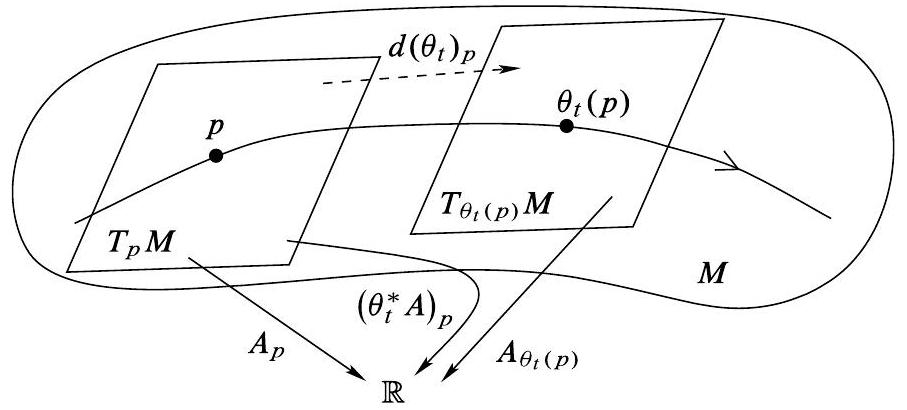
\includegraphics[scale=0.2, center]{2025_06_02_90020b9676379491a6e7g-340}
\end{itemize}

Fig. 12.1 The Lie derivative of a tensor field

Proposition 12.32. Let $M$ be a smooth manifold and let $V \in \mathfrak{X}(M)$. Suppose $f$ is a smooth real-valued function (regarded as a 0 -tensor field) on $M$, and $A, B$ are smooth covariant tensor fields on $M$.\\
(a) $\mathscr{L}_{V} f=V f$.\\
(b) $\mathscr{L}_{V}(f A)=\left(\mathscr{L}_{V} f\right) A+f \mathscr{L}_{V} A$.\\
(c) $\mathscr{L}_{V}(A \otimes B)=\left(\mathscr{L}_{V} A\right) \otimes B+A \otimes \mathscr{L}_{V} B$.\\
(d) If $X_{1}, \ldots, X_{k}$ are smooth vector fields and $A$ is a smooth $k$-tensor field,

$$
\begin{aligned}
\mathscr{L}_{V}\left(A\left(X_{1}, \ldots, X_{k}\right)\right)= & \left(\mathscr{L}_{V} A\right)\left(X_{1}, \ldots, X_{k}\right)+A\left(\mathscr{L}_{V} X_{1}, \ldots, X_{k}\right) \\
& +\cdots+A\left(X_{1}, \ldots, \mathscr{L}_{V} X_{k}\right)
\end{aligned}
$$

Proof. Let $\theta$ be the flow of $V$. For a real-valued function $f$, we can write

$$
\theta_{t}^{*} f(p)=f\left(\theta_{t}(p)\right)=f \circ \theta^{(p)}(t)
$$

Thus the definition of $\mathscr{L}_{V} f$ reduces to the ordinary derivative with respect to $t$ of the composite function $f \circ \theta^{(p)}$. Because $\theta^{(p)}$ is an integral curve of $V$, it follows from Proposition 3.24 that

$$
\left(\mathscr{L}_{V} f\right)(p)=\left.\frac{d}{d t}\right|_{t=0} f \circ \theta^{(p)}=d f_{p}\left(\theta^{(p)^{\prime}}(0)\right)=d f_{p}\left(V_{p}\right)=V f(p) .
$$

This proves (a).\\
The other assertions can be proved by the technique we used in Theorem 9.38: in a neighborhood of a regular point for $V$, if $\left(u^{i}\right)$ are coordinates in which $V=$ $\partial / \partial u^{1}$, then it follows immediately from the definition that $\mathscr{L}_{V}$ acts on a tensor field simply by taking the partial derivative of its coefficients with respect to $u^{1}$, and (b)(d) all follow from the ordinary product rule. The same relations hold on the support of $V$ by continuity, and on the complement of the support because the flow of $V$ is trivial there.

One consequence of this proposition is the following formula expressing the Lie derivative of any smooth covariant tensor field in terms of Lie brackets and ordinary directional derivatives of functions, which allows us to compute Lie derivatives without first determining the flow.

Corollary 12.33. If $V$ is a smooth vector field and $A$ is a smooth covariant $k$-tensor field, then for any smooth vector fields $X_{1}, \ldots, X_{k}$,

$$
\begin{aligned}
\left(\mathscr{L}_{V} A\right)\left(X_{1}, \ldots, X_{k}\right)= & V\left(A\left(X_{1}, \ldots, X_{k}\right)\right)-A\left(\left[V, X_{1}\right], X_{2}, \ldots, X_{k}\right) \\
& -\cdots-A\left(X_{1}, \ldots, X_{k-1},\left[V, X_{k}\right]\right)
\end{aligned}
$$

Proof. Just solve (12.9) for $\left(\mathscr{L}_{V} A\right)\left(X_{1}, \ldots, X_{k}\right)$, and replace $\mathscr{L}_{V} f$ by $V f$ and $\mathscr{L}_{V} X_{i}$ by $\left[V, X_{i}\right]$.

Corollary 12.34. If $f \in C^{\infty}(M)$, then $\mathscr{L}_{V}(d f)=d\left(\mathscr{L}_{V} f\right)$.\\
Proof. Using (12.10), for any $X \in \mathfrak{X}(M)$ we compute

$$
\begin{aligned}
\left(\mathscr{L}_{V} d f\right)(X) & =V(d f(X))-d f([V, X])=V X f-[V, X] f \\
& =V X f-(V X f-X V f)=X V f \\
& =d(V f)(X)=d\left(\mathscr{L}_{V} f\right)(X)
\end{aligned}
$$

One drawback of formula (12.10) is that in order to calculate what $\mathscr{L}_{V} A$ does to vectors $v_{1}, \ldots, v_{k}$ at a point $p \in M$, one must first extend them to vector fields in a neighborhood of $p$. But Proposition 12.32 and Corollary 12.34 lead to an easy method for computing Lie derivatives of smooth tensor fields in coordinates that avoids this problem, since any tensor field can be written locally as a linear combination of functions multiplied by tensor products of exact 1 -forms. The next example illustrates the technique.

Example 12.35. Suppose $A$ is an arbitrary smooth covariant 2 -tensor field, and $V$ is a smooth vector field. We compute the Lie derivative $\mathscr{L}_{V} A$ in smooth local coordinates $\left(x^{i}\right)$. First, we observe that $\mathscr{L}_{V} d x^{i}=d\left(\mathscr{L}_{V} x^{i}\right)=d\left(V x^{i}\right)=d V^{i}$. Therefore,

$$
\begin{aligned}
\mathscr{L}_{V} A & =\mathscr{L}_{V}\left(A_{i j} d x^{i} \otimes d x^{j}\right) \\
& =\mathscr{L}_{V}\left(A_{i j}\right) d x^{i} \otimes d x^{j}+A_{i j}\left(\mathscr{L}_{V} d x^{i}\right) \otimes d x^{j}+A_{i j} d x^{i} \otimes\left(\mathscr{L}_{V} d x^{j}\right) \\
& =V A_{i j} d x^{i} \otimes d x^{j}+A_{i j} d V^{i} \otimes d x^{j}+A_{i j} d x^{i} \otimes d V^{j} \\
& =\left(V A_{i j}+A_{k j} \frac{\partial V^{k}}{\partial x^{i}}+A_{i k} \frac{\partial V^{k}}{\partial x^{j}}\right) d x^{i} \otimes d x^{j}
\end{aligned}
$$

Recall that the Lie derivative of a vector field $W$ with respect to $V$ is zero if and only if $W$ is invariant under the flow of $V$ (see Theorem 9.42). It turns out that the Lie derivative of a covariant tensor field has exactly the same interpretation. If $A$ is a smooth tensor field on $M$ and $\theta$ is a flow on $M$, we say that $\boldsymbol{A}$ is invariant under $\boldsymbol{\theta}$ if for each $t$, the map $\theta_{t}$ pulls $A$ back to itself wherever it is defined; more precisely, this means

$$
d\left(\theta_{t}\right)_{p}^{*}\left(A_{\theta_{t}(p)}\right)=A_{p}
$$

for all ( $t, p$ ) in the domain of $\theta$. If $\theta$ is a global flow, this is equivalent to $\theta_{t}^{*} A=A$ for all $t \in \mathbb{R}$.

In order to prove the connection between Lie derivatives and invariance under flows, we need the following proposition, which shows how the Lie derivative can be used to compute $t$-derivatives at times other than $t=0$. It is a generalization to tensor fields of Proposition 9.41.

Proposition 12.36. Suppose $M$ is a smooth manifold with or without boundary and $V \in \mathfrak{X}(M)$. If $\partial M \neq \varnothing$, assume in addition that $V$ is tangent to $\partial M$. Let $\theta$ be the flow of $V$. For any smooth covariant tensor field $A$ and any ( $t_{0}, p$ ) in the domain of $\theta$,

$$
\left.\frac{d}{d t}\right|_{t=t_{0}}\left(\theta_{t}^{*} A\right)_{p}=\left(\theta_{t_{0}}^{*}\left(\mathscr{L}_{V} A\right)\right)_{p}
$$

Proof. After expanding the definitions of the pullbacks in (12.12), we see that we have to prove

$$
\left.\frac{d}{d t}\right|_{t=t_{0}} d\left(\theta_{t}\right)_{p}^{*}\left(A_{\theta_{t}(p)}\right)=d\left(\theta_{t_{0}}\right)_{p}^{*}\left(\left(\mathscr{L}_{V} A\right)_{\theta_{t_{0}}}(p)\right)
$$

Just as in the proof of Proposition 9.41, the change of variables $t=s+t_{0}$ yields

$$
\begin{aligned}
\left.\frac{d}{d t}\right|_{t=t_{0}} d\left(\theta_{t}\right)_{p}^{*}\left(A_{\theta_{t}(p)}\right) & =\left.\frac{d}{d s}\right|_{s=0} d\left(\theta_{s+t_{0}}\right)_{p}^{*}\left(A_{\theta_{s+t_{0}}}(p)\right) \\
& =\left.\frac{d}{d s}\right|_{s=0} d\left(\theta_{t_{0}}\right)_{p}^{*} d\left(\theta_{s}\right)_{\theta_{t_{0}}(p)}^{*}\left(A_{\theta_{s}\left(\theta_{t_{0}}(p)\right)}\right) \\
& =\left.d\left(\theta_{t_{0}}\right)_{p}^{*} \frac{d}{d s}\right|_{s=0} d\left(\theta_{s}\right)_{\theta_{t_{0}}(p)}^{*}\left(A_{\theta_{s}\left(\theta_{t_{0}}(p)\right)}\right) \\
& =d\left(\theta_{t_{0}}\right)_{p}^{*}\left(\left(\mathscr{L}_{V} A\right)_{\theta_{t_{0}}(p)}\right)
\end{aligned}
$$

Theorem 12.37. Let $M$ be a smooth manifold and let $V \in \mathfrak{X}(M)$. A smooth covariant tensor field $A$ is invariant under the flow of $V$ if and only if $\mathscr{L}_{V} A=0$.

\begin{itemize}
  \item Exercise 12.38. Prove Theorem 12.37.
\end{itemize}

\section*{Problems}
12-1. Give an example of finite-dimensional vector spaces $V$ and $W$ and a specific element $\alpha \in V \otimes W$ that cannot be expressed as $v \otimes w$ for $v \in V$ and $w \in W$.\\
12-2. For any finite-dimensional real vector space $V$, prove that there are canonical isomorphisms $\mathbb{R} \otimes V \cong V \cong V \otimes \mathbb{R}$.\\
12-3. Let $V$ and $W$ be finite-dimensional real vector spaces. Show that the tensor product space $V \otimes W$ is uniquely determined up to canonical isomorphism by its characteristic property (Proposition 12.7). More precisely, suppose $\tilde{\pi}: V \times W \rightarrow Z$ is a bilinear map into a vector space $Z$ with the following


\end{document}